%%%%%%%%%%%%%%%%%%%%%%%%%%%%%%%%%%%%%%%%%%%%%%%%%%%%%%%%%%%%%%%%%%%%%%%%%%%%%%%%
%
% Template license:
% CC BY-NC-SA 3.0 (http://creativecommons.org/licenses/by-nc-sa/3.0/)
%
%%%%%%%%%%%%%%%%%%%%%%%%%%%%%%%%%%%%%%%%%%%%%%%%%%%%%%%%%%%%%%%%%%%%%%%%%%%%%%%%

%----------------------------------------------------------------------------------------
%	PACKAGES AND OTHER DOCUMENT CONFIGURATIONS
%----------------------------------------------------------------------------------------

\documentclass[
11pt, % The default document font size, options: 10pt, 11pt, 12pt
%oneside, % Two side (alternating margins) for binding by default, uncomment to switch to one side
%chapterinoneline,% Have the chapter title next to the number in one single line
spanish,
singlespacing, % Single line spacing, alternatives: onehalfspacing or doublespacing
%draft, % Uncomment to enable draft mode (no pictures, no links, overfull hboxes indicated)
%nolistspacing, % If the document is onehalfspacing or doublespacing, uncomment this to set spacing in lists to single
%liststotoc, % Uncomment to add the list of figures/tables/etc to the table of contents
%toctotoc, % Uncomment to add the main table of contents to the table of contents
parskip, % Uncomment to add space between paragraphs
%codirector, % Uncomment to add a codirector to the title page
headsepline, % Uncomment to get a line under the header
]{MastersDoctoralThesis} % The class file specifying the document structure



%----------------------------------------------------------------------------------------
%	INFORMACIÓN DE LA MEMORIA
%----------------------------------------------------------------------------------------

\thesistitle{PIDS: Sistema de información visual para pasajeros de Trenes Argentinos} % El títulos de la memoria, se usa en la carátula y se puede usar el cualquier lugar del documento con el comando \ttitle

% Nombre del posgrado, se usa en la carátula y se puede usar el cualquier lugar del documento con el comando \degreename
\posgrado{Carrera de Especialización en Sistemas Embebidos} 
%\posgrado{Carrera de Especialización en Internet de las Cosas} 
%\posgrado{Carrera de Especialización en Intelegencia Artificial}
%\posgrado{Maestría en Sistemas Embebidos} 
%\posgrado{Maestría en Internet de las cosas}

\author{Ing. Carlos German Carreño Romano} % Tu nombre, se usa en la carátula y se puede usar el cualquier lugar del documento con el comando \authorname

\director{Dr. Ing. Pablo Martín Gomez (UBA)} % El nombre del director, se usa en la carátula y se puede usar el cualquier lugar del documento con el comando \dirname
\codirector{Nombre del codirector (pertenencia)} % El nombre del codirector si lo hubiera, se usa en la carátula y se puede usar el cualquier lugar del documento con el comando \codirname.  Para activar este campo se debe descomentar la opción "codirector" en el comando \documentclass, línea 23.

\juradoUNO{Nombre del jurado 1 (pertenencia)} % Nombre y pertenencia del un jurado se usa en la carátula y se puede usar el cualquier lugar del documento con el comando \jur1name
\juradoDOS{Nombre del jurado 2 (pertenencia)} % Nombre y pertenencia del un jurado se usa en la carátula y se puede usar el cualquier lugar del documento con el comando \jur2name
\juradoTRES{Nombre del jurado 3 (pertenencia)} % Nombre y pertenencia del un jurado se usa en la carátula y se puede usar el cualquier lugar del documento con el comando \jur3name

\ciudad{Ciudad Autónoma de Buenos Aires}
%\ciudad{ciudad de Mendoza}

\fechaINICIO{marzo de 2020}
\fechaFINAL{diciembre de 2023}


\keywords{Sistemas embebidos, FIUBA} % Keywords for your thesis, print it elsewhere with \keywordnames

\begin{document}


\frontmatter % Use roman page numbering style (i, ii, iii, iv...) for the pre-content pages

\pagestyle{plain} % Default to the plain heading style until the thesis style is called for the body content


%----------------------------------------------------------------------------------------
%	RESUMEN - ABSTRACT 
%----------------------------------------------------------------------------------------

\begin{abstract}
\addchaptertocentry{\abstractname} % Add the abstract to the table of contents
%
%The Thesis Abstract is written here (and usually kept to just this page). The page is kept centered vertically so can expand into the blank space above the title too\ldots
\centering

En este trabajo se aborda el desarrollo de un sistema de información visual para pasajeros para la empresa Trenes Argentinos. Las formaciones ferroviarias tienen carteles de matriz led dentro de los coches por donde se comunican mensajes tales como la próxima estación. Estos carteles forman parte de una red de comunicaciones que interconecta distintos sistemas de control dentro del tren. El sistema desarrollado en este trabajo puede recibir datos de la red de comunicaciones y controlar carteles de matriz led compatibles con los existentes. El sistema sigue una arquitectura orientada a eventos, haciendo uso de técnicas de concurrencia y patrones de software tales como objeto activo, máquinas de estado y gestión de memoria dinámica, sobre un sistema operativo de tiempo real. Se han realizado ensayos y mediciones en trenes operativos, que han proporcionado tramas de datos reales que fueron analizadas para usarse como entradas del sistema. En la región del  AMBA, los trenes operan aproximadamente con 500 carteles del mismo modelo de forma simultánea. Estos suelen presentar fallas, y su reemplazo se ve dificultado por problemas de importación. Con este trabajo se pretende contribuir a la sustitución de las placas de control y al mantenimiento de las unidades, con el fin de extender la vida útil de los trenes. 

\end{abstract}

%----------------------------------------------------------------------------------------
%	CONTENIDO DE LA MEMORIA  - AGRADECIMIENTOS
%----------------------------------------------------------------------------------------

\begin{acknowledgements}
%\addchaptertocentry{\acknowledgementname} % Descomentando esta línea se puede agregar los agradecimientos al índice
\vspace{1.5cm}

En primer lugar, quiero agradecer al Dr. Ing. Pablo Gomez por su inagotable paciencia y excelente predisposición a lo largo de todo el tiempo que llevó concluir este trabajo. También quiero agradecer al Dr. Ing. Ariel Lutenberg por su empuje, su espíritu motivador y su actitud de concertación. Me gustaría destacar su liderazgo en la generación de propuestas concretas de vinculación entre la universidad y la industria a través de proyectos de desarrollo de tecnología. Quiero reconocer el valioso aporte de ambos y del cuerpo docente que han volcado a lo largo de los años un enorme y minucioso trabajo en el desarrollo de los contenidos del programa de la Carrera de Especialización en Sistemas Embebidos. Ha sido altamente satisfactorio completar el posgrado.

Asimismo, me gustaría agradecer al personal altamente calificado de la Gerencia de Material Rodante Eléctrico de la companía Trenes Argentinos Operaciones (SOFSE), el Ing. Sergio Dieleke, y a todos los colaboradores que nos han brindado atención, seguridad y tiempo para realizar mediciones en las formaciones ferroviarias. Quiero hacer una mención especial de reconocimiento a Bruno Pilato por su colaboración desde los talleres de Castelar para realizar pruebas en conjunto durante la etapa de confinamiento debido a la pandemia. 

Por último, también agradezco a Magui, que me brindó soporte en 
todo momento; a mi madre y a mi padre por enseñarme a valorar tanto la formación académica como la experiencia técnica con igual importancia; y a mis tutores y colegas de la empresa con quienes comparto el día a día e intercambio ideas sumamente útiles para pensar fuera de la caja.


\end{acknowledgements}

%----------------------------------------------------------------------------------------
%	LISTA DE CONTENIDOS/FIGURAS/TABLAS
%----------------------------------------------------------------------------------------

\tableofcontents % Prints the main table of contents

%\listoffigures % Prints the list of figures

%\listoftables % Prints the list of tables


%----------------------------------------------------------------------------------------
%	CONTENIDO DE LA MEMORIA  - DEDICATORIA
%----------------------------------------------------------------------------------------

%\dedicatory{\textbf{Dedicado a la Facultad de Ingeniería de la Universidad de Buenos Aires y a la empresa Trenes Argentinos Operaciones}}  % escribir acá si se desea una dedicatoria

%----------------------------------------------------------------------------------------
%	CONTENIDO DE LA MEMORIA  - CAPÍTULOS
%----------------------------------------------------------------------------------------

\mainmatter % Begin numeric (1,2,3...) page numbering

\pagestyle{thesis} % Return the page headers back to the "thesis" style

% Incluir los capítulos como archivos separados desde la carpeta Chapters

%----------------------------------------------------------------------------------------

% Define some commands to keep the formatting separated from the content 
\newcommand{\keyword}[1]{\textbf{#1}}
\newcommand{\tabhead}[1]{\textbf{#1}}
\newcommand{\code}[1]{\texttt{#1}}
\newcommand{\file}[1]{\texttt{\bfseries#1}}
\newcommand{\option}[1]{\texttt{\itshape#1}}
\newcommand{\grados}{$^{\circ}$}

%----------------------------------------------------------------------------------------
%\section{Introducción}
%----------------------------------------------------------------------------------------

% Chapter 1

\chapter{Introducción general} % Main chapter title
\label{Chapter1} % For referencing the chapter elsewhere, use \ref{Chapter1} 
\label{Intro}

Este capítulo introduce al lector a la motivación original del trabajo realizado. Se explica el marco de investigación del que forma parte este proyecto, se presentan los sistemas de información visual y también el estado del arte en controladores de carteles led para estos sistemas.\\

  


%En el capítulo 2 se introduce vocabulario técnico específico. Se presenta una descripción del sistema con el foco en la red de comunicaciones TCN, el sistema PIDS, sus interacciones y componentes.\\
%
%En el capítulo 3 se abordan cuestiones de diseño de sistema. Se especifican los requerimientos y casos de uso que se plantean en el espacio problema y también las consideraciones del espacio solución. Se detalla la solución en términos de arquitectura, patrones de software, descripción de componentes e implementación. Se incluye también los planos de los circuitos eléctricos del hardware existente que fueron relevados al realizar este trabajo.\\
%
%En el capítulo 4 se abordan cuestiones relacionadas al entorno real del sistema: visitas técnicas, mediciones realizadas, hardware ad-hoc realizado para las mediciones y un breve análisis de las tramas de datos de la red PIDS existente.\\
%
%En el capítulo 5 se tratan las conclusiones principales del desarrollo, su potencial fabricación en serie y los pasos a seguir para integrar al resto de ramales ferroviarios. En el apéndice de bibliografía se encontrarán las principales referencias técnicas, científicas e institucionales relevantes para este trabajo.\\


\section{Descripción del trabajo}

En este trabajo se desarrolla el sistema de control para carteles de matriz led del sistema de información visual para pasajeros (PIDS) de Trenes Argentinos. Las formaciones de Trenes Argentinos cuentan con carteles de matriz led en sus coches, en el frente y en el contrafrente del tren. Todos estos carteles se interconectan a través de una red de comunicaciones propia del PIDS, por la que también se transmiten distintos tipos de datos, como datos de mapas led, mensajes de audio, información para los carteles led e incluso videos de cámaras de seguridad. La red PIDS convive y se interconecta con la red de comunicaciones del tren (TCN), que es una red estándar. Además, en los buses de datos de la red TCN, se transmiten datos de sensores de velocidad, de frenado y eventos que indican apertura o cierre de puertas, entre otros. \\

Los carteles led del sistema PIDS suelen presentar fallas a lo largo de su ciclo de vida, lo que implica tareas de mantenimiento, reparación o reposición. Si bien existen muchos tipos de carteles led disponibles comercialmente, la integración al sistema de comunicaciones del tren es propietaria del fabricante de trenes. Para el caso de Trenes Argentinos, el proveedor está radicado en China, lo que hace muy costoso y lento el proceso de reposición o mantenimiento de equipamiento. Por esta razón, el desarrollo local de tecnología para sistemas PIDS es estratégico, ya que no solo fomenta la industria local, sino que también extiende la vida útil de los trenes.\\

%Esta necesidad motiva el desarrollo como búsqueda de autonomía tecnológica en áreas de vacancia que pueden ser cubiertas por el sistema científico-tecnológico nacional.

El eje de este trabajo es el desarrollo de un sistema a medida para Trenes Argentinos. La necesidad que prima es generar y brindar al personal de operaciones la información necesaria para construir y mantener los sistemas PIDS. Como resultado, este trabajo también tiene impacto directo en el pasajero, ya que contribuye a mejorar la calidad del servicio.\\


%\pagebreak
\section{Objetivos y alcance}

El  contexto de este trabajo se encuentra enmarcado en un Proyecto de Desarrollo Estratégico (PDE) de la Secretaría de Ciencia y Técnica de la Universidad de Buenos Aires (UBACyT). El PDE se titula PDE\_15\_2020 - "Sistema de monitoreo y gestión de la red TCN en formaciones ferroviarias"\ \citep{PDE-TCN}. Las partes que se involucran y forman parte del equipo de trabajo en este proyecto son el Grupo de Investigación en Calidad y Seguridad de las Aplicaciones Ferroviarias (GICSAFE), creado en 2017 en el marco del Consejo Nacional de Investigaciones Científicas y Técnicas (CONICET) de la República Argentina, y la  Operadora Ferroviaria Sociedad del Estado (SOFSE), también conocida como Trenes Argentinos Operaciones. El proyecto está orientado a cubrir necesidades tecnológicas concretas del sistema ferroviario argentino. Este tipo de proyectos son instrumentos de promoción científico-tecnológica que revalorizan e incrementan el aporte de la Universidad al desarrollo socioproductivo.\\

El objetivo principal de este trabajo es diseñar e implementar un sistema de información visual para pasajeros a bordo del tren. El sistema de información visual para pasajeros existente consta de una parte manual y una automática. Cuando el conductor del tren asume su puesto para prestar servicio (o toma cabina), programa en una pantalla cuáles van a ser las estaciones cabecera. Los nombres de estas estaciones cabecera se visualizan en las marquesinas del frente y contrafrente del tren, como puede verse en la figura \ref{fig:tren}.

\begin{figure}[ht]
	\centering
	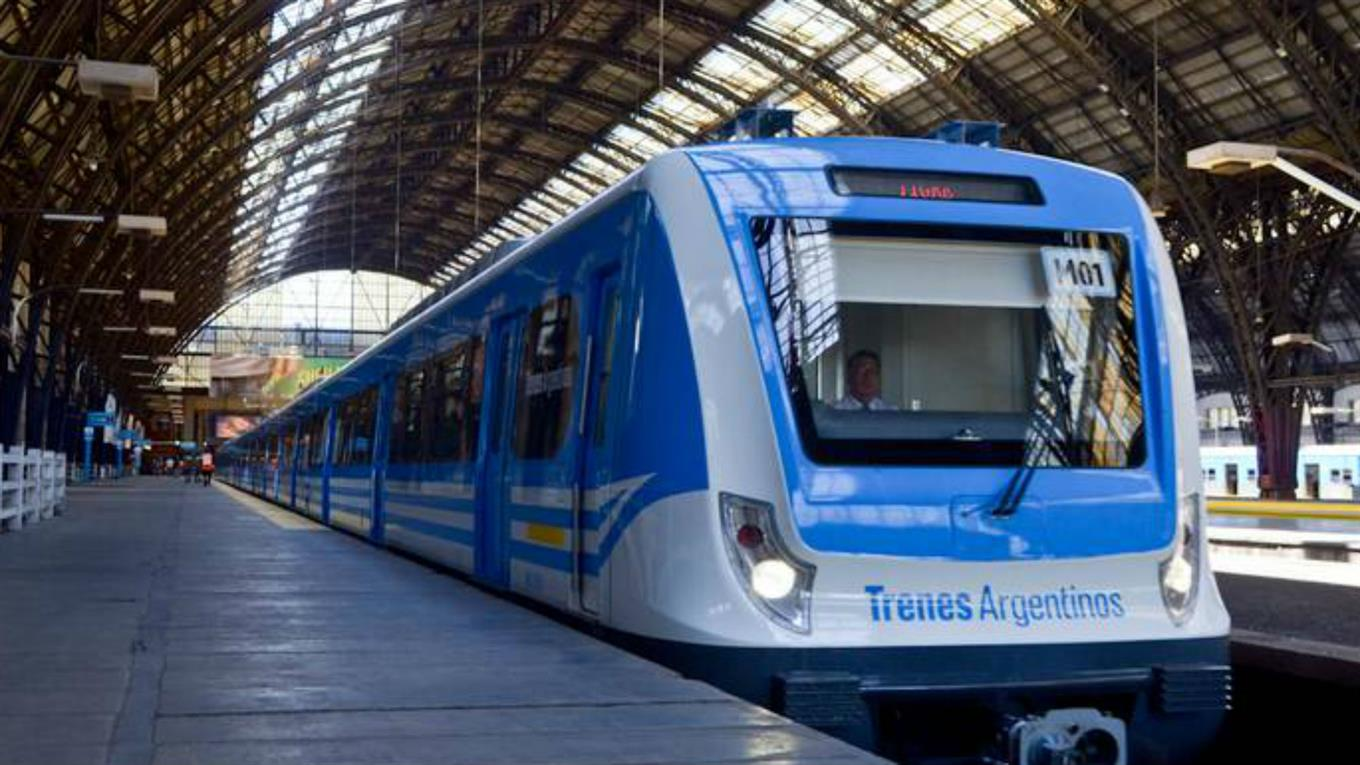
\includegraphics[width=1\textwidth]{./Figures/tren.jpg}
	\caption{Foto de una formación operativa de Trenes Argentinos. Se observa el cartel de matriz led frontal que indica el destino Tigre.}
	\label{fig:tren}
\end{figure}


En el interior de los coches, también hay carteles led. Estas marquesinas muestran mensajes a los pasajeros, como el nombre de la próxima estación o la estación arribada (por ejemplo, “Próxima estación Belgrano” o “Estás en estación Belgrano”). La información se
presenta de manera automática basándose en variables de sistema que monitorean el detenimiento del tren, su velocidad y la apertura o cierre de puertas. Toda esta información, junto con otros datos de supervisición y control, se transmite a través de una red de comunicación interna del tren que se denomina TCN (\textit{Train Communication Network}) de acuerdo a las especificaciones definidas en el estándar\ \citep{IEC-61375-1999}. Este estándar define para la red TCN dos buses jerárquicos donde se conectan los subsistemas electrónicos: el WTB (\textit{Wire Train Bus}), que se utiliza para supervisar cambios topográficos en el tren y se conecta entre los vagones, y el MVB (\textit{Multi-Vehicle Bus}) \citep{CSN-EN-61375-2-1}\citep{IEC-61375-3-1:2012}, donde se conectan los sensores y actuadores de cada coche, como los sistemas de frenos, los controles de las puertas, los medidores de velocidad, el sistema de información, entre otros. Ambos buses utilizan interfaces eléctricas que se basan en redes RS485.\\


 El sistema propuesto en este trabajo tiene como objetivo captar los mensajes de información al pasajero que viajan por la red existente y presentarlos en un display led. El sistema se compone principalmente de cuatro partes:
 \begin{itemize}
\item Display led.
\item Placa de control.
\item Cableado de interconexión.
\item Firmware del sistema embebido
 \end{itemize}

El diagrama del prototipo se presenta en la figura \ref{fig:diagramaPIDSCIAA}. El display led matricial representa los carteles de los coches del tren. La placa de control se debe poder conectar a la entrada con al bus de la red RS485 que corresponda y a la salida con un display led matricial.

\begin{figure}[ht]
	\centering
	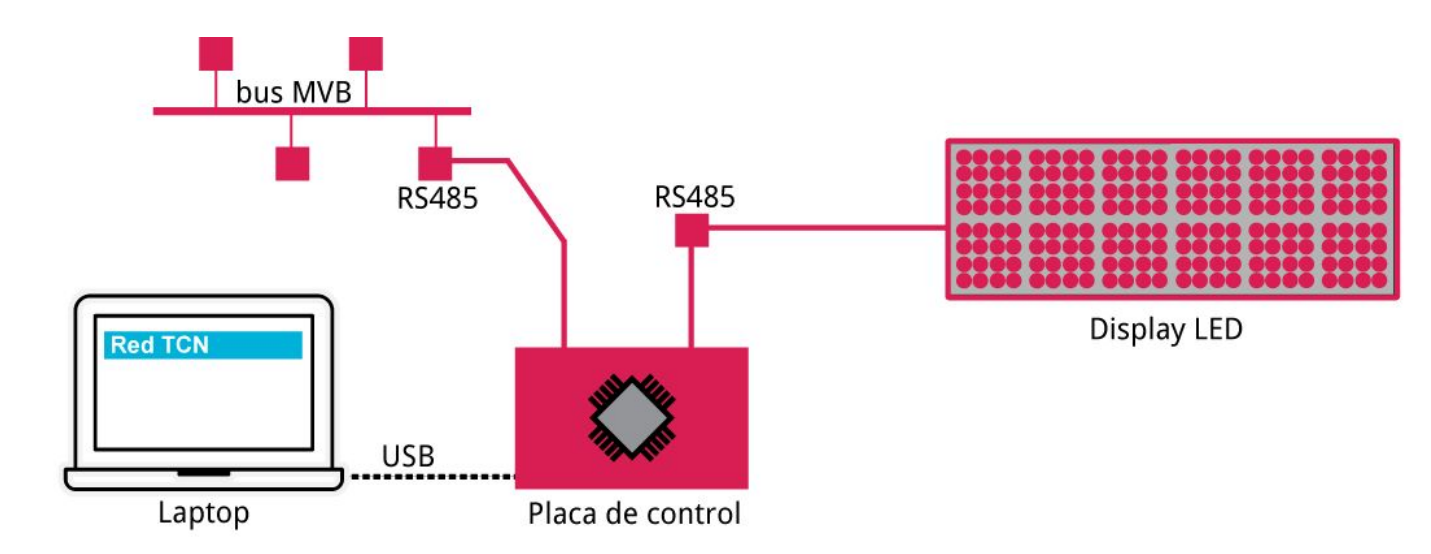
\includegraphics[width=1\textwidth]{./Figures/diagramaPIDSCIAA.png}
	\caption{Diagrama de bloques del sistema embebido propuesto basado en la plataforma EDU-CIAA.}
	\label{fig:diagramaPIDSCIAA}
\end{figure}


La placa de control está basada en la plataforma EDU-CIAA \citep{proyecto-ciaa} o en alguna de las plataformas desarrolladas por el CONICET-GICSAFe. La conexión entre el display y la placa así como de la placa con la red TCN deberá ser compatible con el estándar RS-485, definido como capa física de la red TCN. El
firmware a desarrollar se carga a la placa de control utilizando el puerto USB de una laptop. Este firmware es el responsable de leer los mensajes del sistema de información al pasajero y presentarlos en el display.\\

Las cualidades que debe satisfacer este proyecto son:
\begin{itemize}
\item Compatibilidad: debe ser compatible con el sistema PIDS existente.
\item Practicidad: debe ser de fácil uso para el personal de Trenes Argentinos Operaciones.
\end{itemize}

Este trabajo permitirá implementar las funciones de visualización del sistema de información al pasajero sin depender del equipamiento existente. El sistema actual es un equipamiento integrado y propietario, y este trabajo busca separar algunas de sus funciones, específicamente las relacionadas con la visualización de información para pasajeros, y presentarlas en un display led genérico. Por otro lado, permitirá reponer los carteles que en la actualidad quedan fuera de servicio por fallas o pérdida del material original y no pueden ser reparados. De esta manera, el valor principal que aporta este trabajo es contribuir con la sustitución de repuestos faltantes por medio de desarrollo y reducir la dependencia tecnológica de la empresa con los fabricantes. Este trabajo tiene impacto directo en las formaciones ferroviarias existentes, que brindan servicio a los pasajeros todos los días.\\

\section{Introducción a los sistemas de información visual}

Los sistemas de información visual para pasajeros están presentes en diversas industrias y aplicaciones. Se encargan de proveer información a pasajeros en  movimiento y tienen un rol fundamental en la industria del transporte.\\

 Las personas se trasladan por tierra o aire usando automóviles, ómnibus, subtes, trenes o aviones, entre otros. Los sistemas de información visual presentan necesidades y soluciones distintas en cada caso. Por ejemplo, en autopistas, se comunican accidentes u obras viales en ejecución usando carteles gigantes con información en tiempo real. En aeropuertos, los pasajeros aéreos acceden a información sobre llegada, el estado o la salida de vuelos. A los pasajeros de ómnibus, les interesa conocer los tiempos de espera y las líneas en operación al llegar a una estación. Los pasajeros de trenes utilizan estos sistemas para conocer el destino o la próxima estación cuando están viajando. Estos carteles pueden estar ubicados al aire libre o dentro de un recinto, pero en general,  requieren estar sincronizados con los vehículos en movimiento. \\

Los sistemas de información visual para pasajeros, constan principalmente de tres componentes: un sistema que genera datos, una red de transmisión y un sistema de pantallas. Las especificaciones de cada sistema varían según el ámbito de aplicación. Típicamente, en los trenes se requiere comunicación en tiempo real, lo que conlleva la adopción de protocolos de datos de tiempo real (RTP). En aplicaciones ferroviarias, también es fundamental garantizar la integridad, disponibilidad y confiabilidad de los datos. Además, existen otros requerimientos de carácter operativo, como el mantenimiento y la facilidad de instalación. Estos últimos aspectos son esenciales en la operación de una formación ferroviaria y tienen impacto directo en el ciclo de vida de un tren.\\

 Los sistemas PIDS instalados en los trenes se interconectan con una red TCN. Ésta última, sigue un estándar que define tanto las interfaces eléctricas como los protocolos de comunicación. En la red TCN, se conectan dispositivos para el sensado y control de frenos, de puertas, de monitoreo, entre otros, usando una arquitectura jerárquica de buses de datos. La red TCN representa un estándar robusto, maduro, probado y con gran adopción internacional. Sin embargo, los sistemas PIDS se presentan sin la necesidad de ser compatibles con los estándares de TCN, al menos hasta la revisión del año 2005. Existen diversas soluciones comerciales de sistemas PIDS, para aplicaciones de entretenimiento por ejemplo, pero se requiere de un trabajo de integración adicional para que funcionen en un tren.\\
 
 En este trabajo se introduce una breve descripción de las redes TCN y su evolución en el tiempo. Para el caso de las formaciones de Trenes Argentinos, se presenta también el detalle de interconexión TCN-PIDS, el desarrollo de un sistema de control para los carteles led del sistema PIDS y los resultados de las pruebas de campo realizadas en conjunto con la empresa Trenes Argentinos Operaciones (SOFSE). Se ha organizado esta memoria buscando acercar al lector primero los conceptos principales de la aplicación y luego el detalle técnico del diseño del sistema embebido propuesto. \\

\section{Estado del arte}

En esta breve sección, se resumen algunas características y aspectos comunes de los sistemas PIDS, tanto para sistemas ferroviarios como para sistemas de transporte integrados. En lugar de ser un estudio sistemático, la intención es guiar al lector en las consideraciones que fueron tenidas en cuenta en este trabajo. En primer lugar, se describe el rol que juegan estos sistemas y una noción de su mercado, mencionando aquellos proveedores que se consideraron relevantes por claridad en la información, marca global y diseño conceptual de la solución. Luego, se describen algunas soluciones comerciales innovadoras, y finalmente se presenta en tablas algunos aspectos técnicos comunes en distintas soluciones. Adicionalmente, se mencionan algunos trabajos académicos relevados. Se han elegido como dimensiones de análisis las funcionalidades y servicios que debe ofrecer un sistema PIDS, las características principales de la oferta de carteles electrónicos, y por último las características técnicas de las unidades de control. \\


El cliente de mayor impacto de los servicios que provee un sistema PIDS es la red de transporte (trenes, subtes, metros, ómnibus) de una gran ciudad, debido a su masividad. En términos generales, se observa que las empresas que proveen sistemas PIDS a las redes metropolitanas de transporte de las grandes ciudades lo hacen bajo formatos distintos. Algunas empresas instalan televisores o pantallas de video, otras carteles led, otras incluyen carteles impresos con algún elemento indicador tipo led, o bien leds en forma de flecha mezclándose con la señalización para indicar nombres de estaciones, pantallas led para desplegar publicidad entre mensajes, etcétera. En algunos países, se han realizado esfuerzos durante la última década para que los sistemas PIDS faciliten el acceso a la información del transporte para personas con discapacidades, movilidad reducida y de edad avanzada. Actualmente, estos sistemas se diseñan teniendo en cuenta al pasajero en el centro de todo, buscando ofrecer servicios de información que mejoren la experiencia de viaje.\\

\begin{figure}[h!]
	\centering
	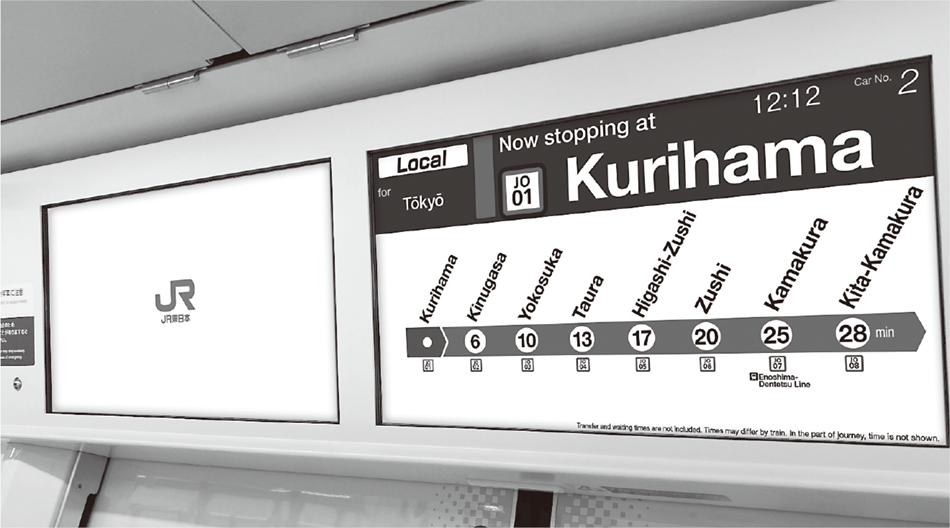
\includegraphics[width=0.49\textwidth]{./Figures/HitachiCartelPIDS.png}
	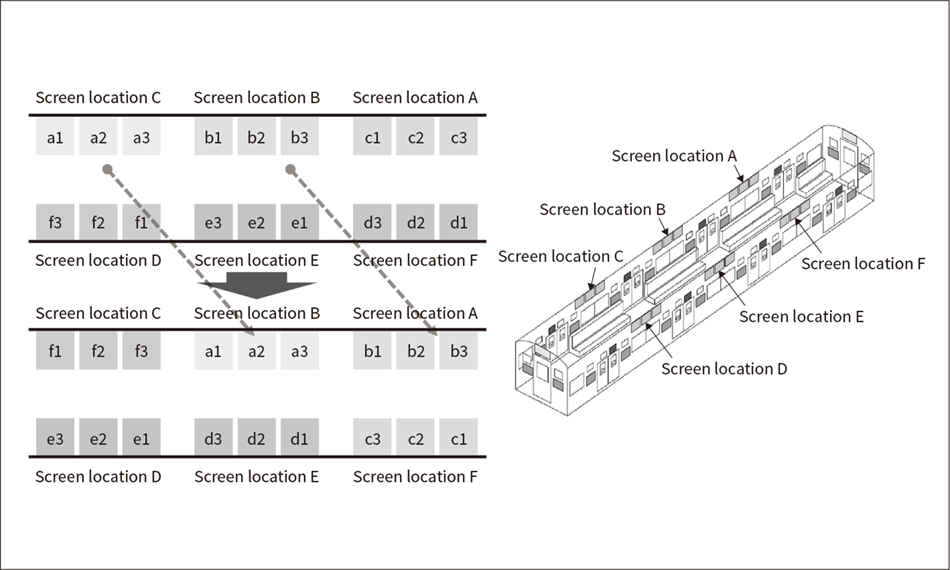
\includegraphics[width=0.49\textwidth]{./Figures/HitachiDisplayArray.png}
	\caption{Solución de carteles para sistemas PIDS de Hitachi.\protect\footnotemark}
	\label{fig:Hitachi}
\end{figure}

\footnotetext{Fuente: consultado en \citep{Hitachi}.}

Hitachi ofrece una solución para publicidad que consiste en tres pantallas en \textit{array}, que se sincronizan para formar una sola y transmitir video con conectividad WiMAX. Cada uno de estos arreglos se posicionan arriba de las ventanas en ambos lados de los coches, alcanzando el despliegue de hasta dieciocho pantallas sincronizadas por coche, como se puede ver en la figura \ref{fig:Hitachi}. De esta manera, logran transmitir varios mensajes distintos en simultáneo a los pasajeros sin que tengan que moverse de su asiento.\\


Por otro lado, Toshiba ofrece una solución que permite transmitir publicidad e información al pasajero en una misma pantalla LCD en simultáneo. La solución está centrada en la pantalla como dispositivo central, ofreciendo pantallas de 32 y 42 pulgadas, de 1920 x 540 píxeles, full color de hasta 16,7 millones de colores, com amplio ángulo de visión y de gran luminancia \citep{Toshiba}. En la mayoría de los casos, las soluciones ofrecidas buscan cubrir tanto la demanda de un sistema PIDS como la oferta de publicidad de cara al pasajero, como es habitual en las estaciones y formaciones ferroviarias.\\



\begin{figure}[h]
	\centering
	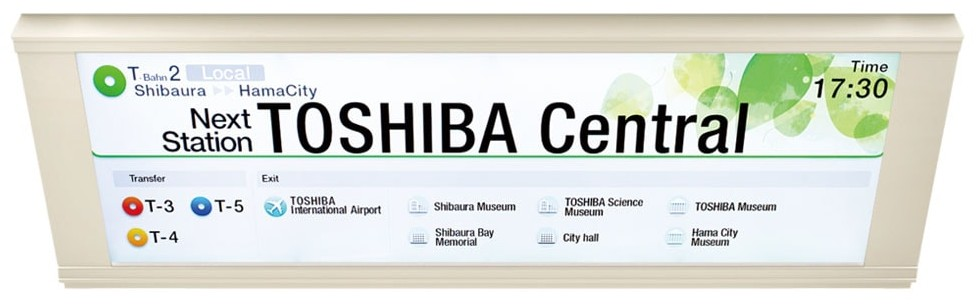
\includegraphics[width=0.49\textwidth]{./Figures/ToshibaPIDS.jpg}
	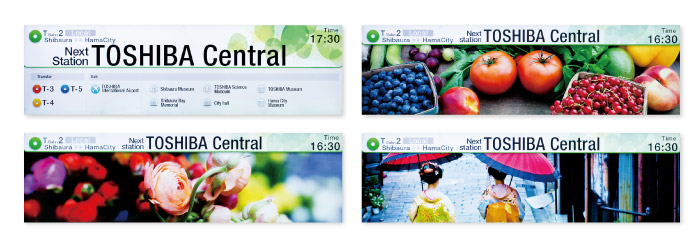
\includegraphics[width=0.49\textwidth]{./Figures/ToshibaDisplayColorOpciones.jpg}
	\caption{Solución de displays LCD para sistemas PIDS de Toshiba.\protect\footnotemark}
	\label{fig:Toshiba}
\end{figure}

\footnotetext{Fuente: consultado en \citep{Toshiba}.}


El grupo austríaco Trapeze \citep{Trapeze} distingue cuatro tecnologías principales en sistemas PIDS: Led, LCD, canales móviles o apps, y e-ink que es una tecnología de LCD monocromo relativamente nueva. Al seleccionar carteles, es importante considerar varios factores, como los ángulos de visión, las condiciones del ambiente donde van instalados (por ejemplo, si estarán a la intemperie o requerirán visibilidad con la luz del sol), el tamaño o resolución de los caracteres en pantalla, la selección de colores y su relación con la capacidad estadística de visión de los pasajeros, el diseño mecánico, el acceso a controles para personas con movilidad reducida, la fuente de alimentación eléctrica y la capacidad de realizar actualizaciones de sistema de forma remota. \\ 


\begin{figure}[h]
	\centering
	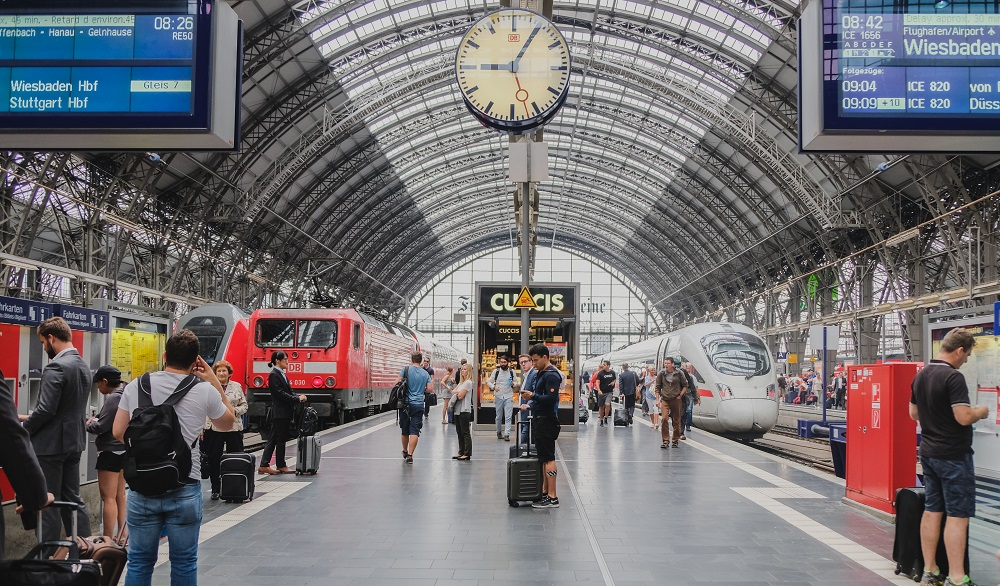
\includegraphics[width=0.32\textwidth]{./Figures/TrapezeStation.jpg}
	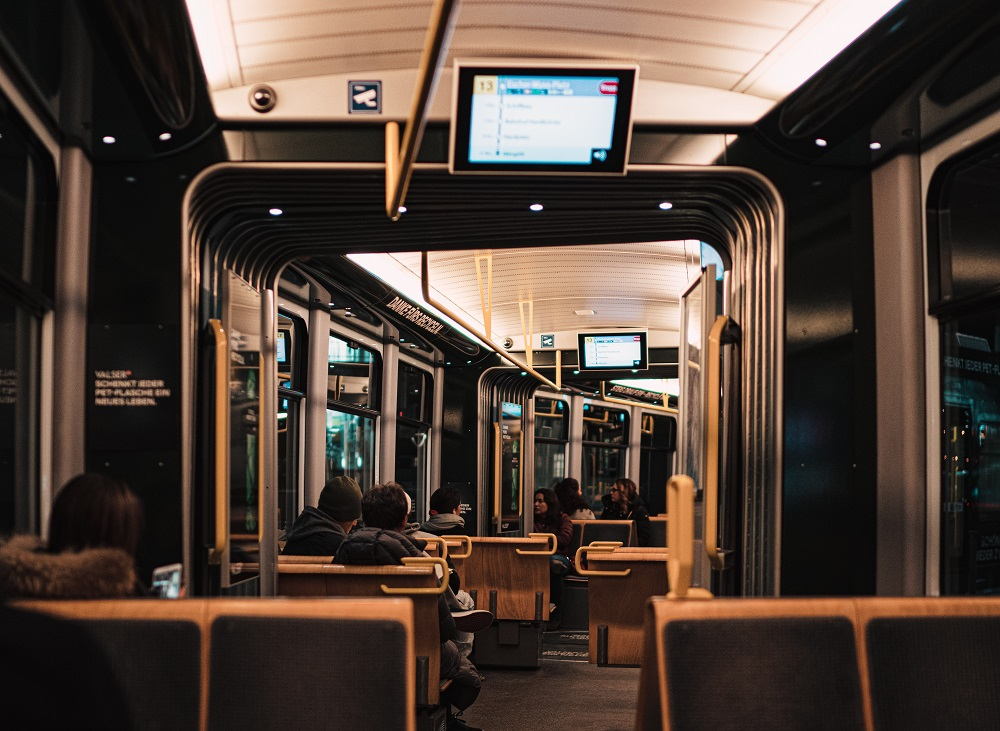
\includegraphics[width=0.32\textwidth]{./Figures/TrapezeOnboard.jpg}
	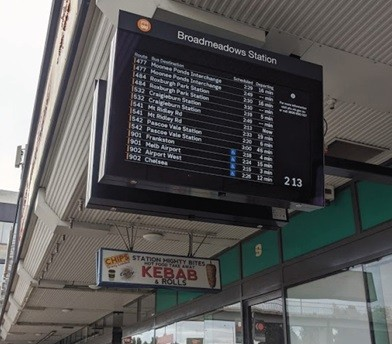
\includegraphics[width=0.32\textwidth]{./Figures/TrapezeTimetable.jpg}
	\caption{Sistema PIDS del proveedor austríaco Trapeze. \protect\footnotemark}
	\label{fig:Trapeze}
\end{figure}

\footnotetext{Fuente: consultado en \citep{Trapeze}.}

Además, se sugiere la importancia de la precisión en la información que ofrece como servicio el sistema PIDS. Si un pasajero recibe el número de andén incorrecto al llegar a la estación muy probablemente perderá el tren, resultando en una mala experiencia de viaje. La capacidad de interconectar el sistema PIDS con otros canales de información, especialmente en puntos nodales de transporte, también ofrece mayores beneficios al usuario final. Si un pasajero puede anticiparse y ver el tiempo estimado entre una línea de omnibus o de tren antes de llegar a la estación donde hace combinación, entonces puede tomar una mejor elección basada en datos ofrecidos por el sistema PIDS. Estos y otros aspectos de sistema centrados en el usuario se resumen en la tabla \ref{tab:tablaSistemasPIDS}.\\

\begin{table}[H]
\caption[Caption for LOF]{Principales aspectos y servicios asociados a sistemas PIDS.\protect\footnotemark}
%\caption{Principales aspectos y servicios asociados a sistemas PIDS\footnote{Elaboración del autor.}.}
\begin{center}
\begin{tabular}{cl}
\toprule
\textbf{Atributo} &\begin{tabular}[c]{@{}l@{}}
    \textbf{Tipo de servicios}                      \\
\end{tabular}\\
\midrule
\textbf{Conectividad} &\begin{tabular}[c]{@{}l@{}}
    RS-485, serial, USB.                    \\
    Ethernet, fibra óptica, coaxil.         \\
    Wi-Fi, WiMax, GPS. 2G / 3G / 4G / 5G.   \\
\end{tabular}\\
\midrule
\textbf{Interconexión} &\begin{tabular}[c]{@{}l@{}}
    App del tren, horarios programados.     \\
    Ómnibus, información multinodal.        \\
    Portales de noticias, publicidad.       \\
    Canal de información estatal.           \\
\end{tabular}\\ 
\midrule
\textbf{Accesibilidad} &\begin{tabular}[c]{@{}l@{}}
    Información por audio, ángulos de visión de los carteles. \\
    Facilidades para personas en sillas de ruedas. \\
    Facilidades para personas de edad avanzada. \\
    Correcto y cuidado sistema de señalización. \\
\end{tabular}\\ 
\midrule
\textbf{Información} &\begin{tabular}[c]{@{}l@{}}
   Estimación de tiempos y aviso de cortes en tiempo real.\\
   Correcto trackeo de vehículos y conexiones.            \\
   Mensajes de alerta o precauciones, números de emergencia.\\
\end{tabular}\\ 
\midrule
\textbf{Mantenibilidad} &\begin{tabular}[c]{@{}l@{}}
   Fácil instalación, bajo costo de reposición.\\
   Consumo eléctrico.                          \\
   Actualizaciones de software.                \\
\end{tabular}\\ 
\bottomrule
\end{tabular}
\label{tab:tablaSistemasPIDS}
\end{center}
\end{table}



Desde el punto de vista centrado en los carteles, se consideran varias especificaciones importantes de los sistemas PIDS, como las dimensiones del cartel, la densidad de píxeles por unidad de área, la cantidad de colores o leds por píxel, los niveles de intensidad lumínica, el brillo y contraste, la potencia eléctrica. Entre estas especificaciones típicas de los carteles de los sistemas PIDS, el ángulo de visión es una de las variables más consideradas ya que en sistemas PIDS implican el alcance a mayor cantidad de pasajeros de la información en pantalla. En la tabla \ref{tab:tablaDisplays} se presenta un resumen de estas características. Las fuentes consultadas para la elaboración de esta tabla son diversos portales internacionales de distribución de componentes electrónicos.\\

\footnotetext{Fuente: elaboración propia del autor.}

\begin{table}[htbp]
\caption[Caption for LOF]{Principales características de displays para sistemas PIDS. \protect\footnotemark}
\label{tab:tablaDisplays}
\begin{center}
\begin{tabular}{lllll}
\toprule
\textbf{Display}
    & \textbf{led matricial}      
    & \textbf{led RGB}      
    & \textbf{TFT LCD}   
    & \textbf{LCD RGB}  \\ 
\hline
\textbf{Colores}  
    & \begin{tabular}[c]{@{}l@{}}
        monocromo \\ 
        multicolor \\ 
        (<10 colores)
    \end{tabular} 
    & \begin{tabular}[c]{@{}l@{}}
        desde 256 \\ 
        hasta 16,7 M\\ 
        (típicamente)\end{tabular}   
    & hasta 16,7 M    
    & \begin{tabular}[c]{@{}l@{}}
        16.7M \\ 
        (típicamente)\\ 
        1,000 M\end{tabular}\\ 
\hline
\textbf{\begin{tabular}[c]{@{}l@{}}
Ángulo \\ de visión\end{tabular}}       
    & 110º     
    & 160º   
    & 120º-140º      
    & 178º      \\ 
\hline
\textbf{\begin{tabular}[c]{@{}l@{}}
Intensidad \\ cd/m$^2$\end{tabular}}   
    & 450 
    & 1500-2000       
    & 350 
    & 900 \\ 
\hline
\textbf{\begin{tabular}[c]{@{}l@{}}
Densidad \\ de píxeles\end{tabular}}    
    & \begin{tabular}[c]{@{}l@{}}
        3,9 k\\ 
        27,7 k\\ 
        110 k 
        \end{tabular}    
    & \begin{tabular}[c]{@{}l@{}}
        P16: 3,9 k\\ 
        P12: 6,9 k\\ 
        P10: 10 k\\ 
        P8: 15,6 k\\ 
        P6: 27,7 k\\ 
        P5: 40 k\\ 
        P4: 62,5 k\\ 
        P3: 111 k\\ 
        P2.5: 160 k\\ 
        P2: 250 k
        \end{tabular} 
    & \begin{tabular}[c]{@{}l@{}}
        29 M/m$^2$ \\ 
        Pixel size\\ 
        179 x 192 $\mu$m\end{tabular} 
    & \begin{tabular}[c]{@{}l@{}}
        4,26 M/m$^2$\\ 
        Pixel size \\ 
        484 x 484 $\mu$m\\
        \\ 
        29 M/m$^2$ \\ 
        Pixel size \\ 
        179 x 192 $\mu$m\end{tabular} \\ 
\hline
\textbf{Potencia} 
    & 10 W          
    & 15-316 W   
    & 20 W    
    & 25 W \\ 
\bottomrule
\end{tabular}
\end{center}
\end{table}


\footnotetext{Fuente: elaboración propia del autor.}

Cada cartel requiere de un controlador como interfaz para procesar información y la codifica según la lógica que requiera el tipo de cartel. Los controladores de los carteles de matriz led suelen basarse en circuitos digitales, en microcontroladores de 8, 16 o 32 bits o en FPGA. Las tasas de transmisión de datos requieren señales de clock que pueden variar desde algunos kHz hasta cientos de MHz. Los tamaños del buffer de memoria depende de la cantidad de píxeles que tenga la pantalla. Las interfaces físicas pueden ser periféricos de un microcontrolador, un pin de propósito general o bien puertos USB o HDMI. Los carteles LCD en muchos casos requieren de la transmisión de señales de video. Esto implica mayores costos de implementación que la alternativa led, pero también mayor versatilidad en la programación de contenidos. En la tabla \ref{tab:tablaControladores} se resumen algunas características principales de los requerimientos de los controladores.\\

\begin{table}[htbp]
\caption[Caption for LOF]{Principales características de controladores de uso general para aplicaciones PIDS. \protect\footnotemark}
\label{tab:tablaControladores}
\centering

\begin{center}
\begin{tabular}{llll}
\toprule
\textbf{\begin{tabular}[c]{@{}l@{}}Unidad de \\ procesamiento\end{tabular}} & \textbf{MCU 8/16/32 bits}                                                                       & \textbf{FPGA / ASIC / DSP}                                                        & \textbf{CPU / DSP}                                                                                      \\ \hline
\textbf{Clock}                                                              & 1-200 MHz                                                                                       & 10-250 MHz                                                                        & 1-3 GHz                                                                                                 \\ \hline
\textbf{Memory buffer}                                                      & 1 kB                                                                                            & 1-512 MB                                                                          & 1-10 GB                                                                                                 \\ \hline
\textbf{Conectividad}                                                       & \begin{tabular}[c]{@{}l@{}}UART (1-4)\\ USB (1-2)\\ RS485\\ GPIO (1-20)\\ Ethernet\end{tabular} & \begin{tabular}[c]{@{}l@{}}Pmod\\ I/O pins (20-800)\\ Ethernet\\ USB\end{tabular} & \begin{tabular}[c]{@{}l@{}}USB \\ VGA\\ HDMI\\ DVI\\ display Port\\ PCI / PCI-E\\ Ethernet\end{tabular} \\ \hline
\textbf{Programación}                                                       & C / C++/ Assembly                                                                               & VHDL, Verilog, XML                                                                & \begin{tabular}[c]{@{}l@{}}C, C++, Java, \\ Python, XML\end{tabular}                                    \\ 
\bottomrule
\end{tabular}
\end{center}
\end{table}

\footnotetext{Fuente: elaboración propia del autor.}

Una vez instalados, los sistemas PIDS suelen requerir mantenimiento. Muchas veces hay fallas de hardware, como por ejemplo leds que dejan de funcionar, una fuente de alimentación o una memoria que se debe reemplazar. Otras veces se requieren cambios en el software, por ejemplo actualizar el contenido de un mensaje o bien cambiarlo. Los atributos de mantenibilidad, versatilidad, modularidad y confiabilidad en la implementación pueden tener un impacto económico relevante en la operación de un servicio de transporte. Para líneas de trenes que cuentan con muchas formaciones ferroviarias operando en simultáneo, las tareas de actualización pueden ser muy intensivas en términos de horas de trabajo y requerir también capacitaciones técnicas periódicas al personal de mantenimiento. Incluso no todos los dispositivos pueden recibir actualizaciones en producción, esto es, en la locación física donde funcionan. En muchos casos es necesario desinstalarlos, llevarlos a un centro técnico y actualizarlos fuera de operación, lo que requiere de ventanas de mantenimiento y de tiempos reducidos para realizar tareas que pueden ser susceptibles a errores. Otra forma es enviar un técnico al sitio que pueda conectar algún periférico y actualizar manualmente cada dispositivo.\\

De los trabajos académicos relevados se mencionan aquellos con propuestas del sistema de control que representan distintas tecnologías. En \citep{song2011design} se utiliza el chip AT89C52 para enviar caracteres chinos sobre matrices de 32 x 192 leds de un solo color; en \citep{liu2011design} se implementa una pantalla led RGB de 320 x 240 píxeles que rota 360º, permitiendo visualizar imágenes en color por persistencia de visión; en \citep{kurdthongmee2004design} se desarrollan algoritmos sobre FPGA usando búferes de datos para controlar una pantalla led de 160 x 32 píxeles alcanzando 32.768 colores; en \citep{lin2021active} se presenta el control de un micro display de transistores de película delgada (TFT) usando modulación por ancho de pulso (PWM) alcanzando 256 niveles de color a una frecuencia de refresco de 60 Hz, basado también en FPGA; en \citep{gago2009control} se presenta el control de píxeles virtuales para matrices led multicolor usando flip-flops tipo D. \\


En el diseño e implementación del presente trabajo, los carteles son de matriz led de un solo color y de distintas dimensiones (8 x 64, 32 x 64, 32 x 128). El control de los carteles tiene como factor común el uso del conjunto de chips digitales 74HC138, 74HC595 y 74HC245. La topología permite interconectar paneles en serie para construir carteles led de distinto tamaño usando la misma lógica de control. \\



\chapter{Introducción específica} % Main chapter title

\label{Chapter2}

%----------------------------------------------------------------------------------------
%	SECTION 1
%----------------------------------------------------------------------------------------
Todos los capítulos deben comenzar con un breve párrafo introductorio que indique cuál es el contenido que se encontrará al leerlo.  La redacción sobre el contenido de la memoria debe hacerse en presente y todo lo referido al proyecto en pasado, siempre de modo impersonal.

\section{Estilo y convenciones}
\label{sec:ejemplo}

\subsection{Uso de mayúscula inicial para los título de secciones}

Si en el texto se hace alusión a diferentes partes del trabajo referirse a ellas como capítulo, sección o subsección según corresponda. Por ejemplo: ``En el capítulo \ref{Chapter1} se explica tal cosa'', o ``En la sección \ref{sec:ejemplo} se presenta lo que sea'', o ``En la subsección \ref{subsec:ejemplo} se discute otra cosa''.

Cuando se quiere poner una lista tabulada, se hace así:

\begin{itemize}
	\item Este es el primer elemento de la lista.
	\item Este es el segundo elemento de la lista.
\end{itemize}

Notar el uso de las mayúsculas y el punto al final de cada elemento.

Si se desea poner una lista numerada el formato es este:

\begin{enumerate}
	\item Este es el primer elemento de la lista.
	\item Este es el segundo elemento de la lista.
\end{enumerate}

Notar el uso de las mayúsculas y el punto al final de cada elemento.

\subsection{Este es el título de una subsección}
\label{subsec:ejemplo}

Se recomienda no utilizar \textbf{texto en negritas} en ningún párrafo, ni tampoco texto \underline{subrayado}. En cambio sí se debe utilizar \textit{texto en itálicas} para palabras en un idioma extranjero, al menos la primera vez que aparecen en el texto. En el caso de palabras que estamos inventando se deben utilizar ``comillas'', así como también para citas textuales. Por ejemplo, un \textit{digital filter} es una especie de ``selector'' que permite separar ciertos componentes armónicos en particular.

La escritura debe ser impersonal. Por ejemplo, no utilizar ``el diseño del firmware lo hice de acuerdo con tal principio'', sino ``el firmware fue diseñado utilizando tal principio''. 

El trabajo es algo que al momento de escribir la memoria se supone que ya está concluido, entonces todo lo que se refiera a hacer el trabajo se narra en tiempo pasado, porque es algo que ya ocurrió. Por ejemplo, "se diseñó el firmware empleando la técnica de test driven development".

En cambio, la memoria es algo que está vivo cada vez que el lector la lee. Por eso transcurre siempre en tiempo presente, como por ejemplo:

``En el presente capítulo se da una visión global sobre las distintas pruebas realizadas y los resultados obtenidos. Se explica el modo en que fueron llevados a cabo los test unitarios y las pruebas del sistema''.

Se recomienda no utilizar una sección de glosario sino colocar la descripción de las abreviaturas como parte del mismo cuerpo del texto. Por ejemplo, RTOS (\textit{Real Time Operating System}, Sistema Operativo de Tiempo Real) o en caso de considerarlo apropiado mediante notas a pie de página.

Si se desea indicar alguna página web utilizar el siguiente formato de referencias bibliográficas, dónde las referencias se detallan en la sección de bibliografía de la memoria, utilizado el formato establecido por IEEE en \citep{IEEE:citation}. Por ejemplo, ``el presente trabajo se basa en la plataforma EDU-CIAA-NXP \citep{CIAA}, la cual...''.

\subsection{Figuras} 

Al insertar figuras en la memoria se deben considerar determinadas pautas. Para empezar, usar siempre tipografía claramente legible. Luego, tener claro que \textbf{es incorrecto} escribir por ejemplo esto: ``El diseño elegido es un cuadrado, como se ve en la siguiente figura:''

\begin{figure}[h]
\centering

\includegraphics[scale=.45]{./Figures/cuadradoAzul.png}
\end{figure}

La forma correcta de utilizar una figura es con referencias cruzadas, por ejemplo: ``Se eligió utilizar un cuadrado azul para el logo, como puede observarse en la figura \ref{fig:cuadradoAzul}''.

\begin{figure}[ht]
	\centering
	
\includegraphics[scale=.45]{./Figures/cuadradoAzul.png}
	\caption{Ilustración del cuadrado azul que se eligió para el diseño del logo.}
	\label{fig:cuadradoAzul}
\end{figure}

El texto de las figuras debe estar siempre en español, excepto que se decida reproducir una figura original tomada de alguna referencia. En ese caso la referencia de la cual se tomó la figura debe ser indicada en el epígrafe de la figura e incluida como una nota al pie, como se ilustra en la figura \ref{fig:palabraIngles}.

\begin{figure}[htpb]
	\centering
	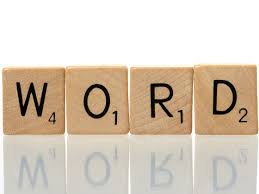
\includegraphics[scale=.3]{./Figures/word.jpeg}
	\caption{Imagen tomada de la página oficial del procesador\protect\footnotemark.}
	\label{fig:palabraIngles}
\end{figure}

\footnotetext{Imagen tomada de \url{https://goo.gl/images/i7C70w}}

La figura y el epígrafe deben conformar una unidad cuyo significado principal pueda ser comprendido por el lector sin necesidad de leer el cuerpo central de la memoria. Para eso es necesario que el epígrafe sea todo lo detallado que corresponda y si en la figura se utilizan abreviaturas entonces aclarar su significado en el epígrafe o en la misma figura.



\begin{figure}[ht]
	\centering
	
\includegraphics[scale=.37]{./Figures/questionMark.png}
	\caption{¿Por qué de pronto aparece esta figura?}
	\label{fig:questionMark}
\end{figure}

Nunca colocar una figura en el documento antes de hacer la primera referencia a ella, como se ilustra con la figura \ref{fig:questionMark}, porque sino el lector no comprenderá por qué de pronto aparece la figura en el documento, lo que distraerá su atención.

Otra posibilidad es utilizar el entorno \textit{subfigure} para incluir más de una figura, como se puede ver en la figura \ref{fig:three graphs}. Notar que se pueden referenciar también las figuras internas individualmente de esta manera: \ref{fig:1de3}, \ref{fig:2de3} y \ref{fig:3de3}.
 
\begin{figure}[!htpb]
     \centering
     \begin{subfigure}[b]{0.3\textwidth}
         \centering
         
\includegraphics[width=.65\textwidth]{./Figures/questionMark}
         \caption{Un caption.}
         \label{fig:1de3}
     \end{subfigure}
     \hfill
     \begin{subfigure}[b]{0.3\textwidth}
         \centering
         
\includegraphics[width=.65\textwidth]{./Figures/questionMark}
         \caption{Otro.}
         \label{fig:2de3}
     \end{subfigure}
     \hfill
     \begin{subfigure}[b]{0.3\textwidth}
         \centering
         
\includegraphics[width=.65\textwidth]{./Figures/questionMark}
         \caption{Y otro más.}
         \label{fig:3de3}
     \end{subfigure}
        \caption{Tres gráficos simples}
        \label{fig:three graphs}
\end{figure}

El código para generar las imágenes se encuentra disponible para su reutilización en el archivo \file{Chapter2.tex}.

\subsection{Tablas}

Para las tablas utilizar el mismo formato que para las figuras, sólo que el epígrafe se debe colocar arriba de la tabla, como se ilustra en la tabla \ref{tab:peces}. Observar que sólo algunas filas van con líneas visibles y notar el uso de las negritas para los encabezados.  La referencia se logra utilizando el comando \verb|\ref{<label>}| donde label debe estar definida dentro del entorno de la tabla.

\begin{verbatim}
\begin{table}[h]
	\centering
	\caption[caption corto]{caption largo más descriptivo}
	\begin{tabular}{l c c}    
		\toprule
		\textbf{Especie}     & \textbf{Tamaño} & \textbf{Valor}\\
		\midrule
		Amphiprion Ocellaris & 10 cm           & \$ 6.000 \\		
		Hepatus Blue Tang    & 15 cm           & \$ 7.000 \\
		Zebrasoma Xanthurus  & 12 cm           & \$ 6.800 \\
		\bottomrule
		\hline
	\end{tabular}
	\label{tab:peces}
\end{table}
\end{verbatim}


\begin{table}[h]
	\centering
	\caption[caption corto]{caption largo más descriptivo}
	\begin{tabular}{l c c}    
		\toprule
		\textbf{Especie} 	 & \textbf{Tamaño} 		& \textbf{Valor}  \\
		\midrule
		Amphiprion Ocellaris & 10 cm 				& \$ 6.000 \\		
		Hepatus Blue Tang	 & 15 cm				& \$ 7.000 \\
		Zebrasoma Xanthurus	 & 12 cm				& \$ 6.800 \\
		\bottomrule
		\hline
	\end{tabular}
	\label{tab:peces}
\end{table}

En cada capítulo se debe reiniciar el número de conteo de las figuras y las tablas, por ejemplo, figura 2.1 o tabla 2.1, pero no se debe reiniciar el conteo en cada sección. Por suerte la plantilla se encarga de esto por nosotros.

\subsection{Ecuaciones}
\label{sec:Ecuaciones}

Al insertar ecuaciones en la memoria dentro de un entorno \textit{equation}, éstas se numeran en forma automática  y se pueden referir al igual que como se hace con las figuras y tablas, por ejemplo ver la ecuación \ref{eq:metric}.

\begin{equation}
	\label{eq:metric}
	ds^2 = c^2 dt^2 \left( \frac{d\sigma^2}{1-k\sigma^2} + \sigma^2\left[ d\theta^2 + \sin^2\theta d\phi^2 \right] \right)
\end{equation}
                                                        
Es importante tener presente que si bien las ecuaciones pueden ser referidas por su número, también es correcto utilizar los dos puntos, como por ejemplo ``la expresión matemática que describe este comportamiento es la siguiente:''

\begin{equation}
	\label{eq:schrodinger}
	\frac{\hbar^2}{2m}\nabla^2\Psi + V(\mathbf{r})\Psi = -i\hbar \frac{\partial\Psi}{\partial t}
\end{equation}

Para generar la ecuación \ref{eq:metric} se utilizó el siguiente código:

\begin{verbatim}
\begin{equation}
	\label{eq:metric}
	ds^2 = c^2 dt^2 \left( \frac{d\sigma^2}{1-k\sigma^2} + 
	\sigma^2\left[ d\theta^2 + 
	\sin^2\theta d\phi^2 \right] \right)
\end{equation}
\end{verbatim}

Y para la ecuación \ref{eq:schrodinger}:

\begin{verbatim}
\begin{equation}
	\label{eq:schrodinger}
	\frac{\hbar^2}{2m}\nabla^2\Psi + V(\mathbf{r})\Psi = 
	-i\hbar \frac{\partial\Psi}{\partial t}
\end{equation}

\end{verbatim} 
\chapter{Desarrollo} % Main chapter title

En este capítulo se presentan los requerimientos del sistema y la solución propuesta. En el desarrollo se utiliza la plataforma de hardware EDU-CIAA\cite{CIAA}, la API Firmware\_ v3\cite{firmwareV3}, y freeRTOS\cite{freeRTOS} como sistema operativo de tiempo real.\\

Se presenta el desarrollo siguiendo lineamientos de ingeniería de software en el siguiente orden: requerimientos, funcionalidades y casos de uso principales como ejes del espacio problema; arquitectura, patrones de software involucrados, técnicas de concurrencia, diagramas de secuencia, de interacción entre componentes, organización del firmware y planos de hardware para describir el espacio solución.\\


\label{Chapter3} % Change X to a consecutive number; for referencing this chapter elsewhere, use \ref{ChapterX}

\definecolor{mygreen}{rgb}{0,0.6,0}
\definecolor{mygray}{rgb}{0.95,0.95,0.95}
\definecolor{mygray50}{rgb}{0.5,0.5,0.5}
\definecolor{mymauve}{rgb}{0.58,0,0.82}

%%%%%%%%%%%%%%%%%%%%%%%%%%%%%%%%%%%%%%%%%%%%%%%%%%%%%%%%%%%%%%%%%%%%%%%%%%%%%
% parámetros para configurar el formato del código en los entornos lstlisting
%%%%%%%%%%%%%%%%%%%%%%%%%%%%%%%%%%%%%%%%%%%%%%%%%%%%%%%%%%%%%%%%%%%%%%%%%%%%%
\lstset{ %
  backgroundcolor=\color{mygray},   % choose the background color; you must add \usepackage{color} or \usepackage{xcolor}
  basicstyle=\footnotesize,        % the size of the fonts that are used for the code
  breakatwhitespace=false,         % sets if automatic breaks should only happen at whitespace
  breaklines=true,                 % sets automatic line breaking
  captionpos=b,                    % sets the caption-position to bottom
  commentstyle=\color{mygreen},    % comment style
  deletekeywords={...},            % if you want to delete keywords from the given language
  %escapeinside={\%*}{*)},          % if you want to add LaTeX within your code
  %extendedchars=true,              % lets you use non-ASCII characters; for 8-bits encodings only, does not work with UTF-8
  %frame=single,	                % adds a frame around the code
  keepspaces=true,                 % keeps spaces in text, useful for keeping indentation of code (possibly needs columns=flexible)
  keywordstyle=\color{blue},       % keyword style
  language=[ANSI]C,                % the language of the code
  %otherkeywords={*,...},           % if you want to add more keywords to the set
  numbers=left,                    % where to put the line-numbers; possible values are (none, left, right)
  numbersep=5pt,                   % how far the line-numbers are from the code
  numberstyle=\tiny\color{mygray50}, % the style that is used for the line-numbers
  rulecolor=\color{black},         % if not set, the frame-color may be changed on line-breaks within not-black text (e.g. comments (green here))
  showspaces=false,                % show spaces everywhere adding particular underscores; it overrides 'showstringspaces'
  showstringspaces=false,          % underline spaces within strings only
  showtabs=false,                  % show tabs within strings adding particular underscores
  stepnumber=1,                    % the step between two line-numbers. If it's 1, each line will be numbered
  stringstyle=\color{mymauve},     % string literal style
  tabsize=2,	                   % sets default tabsize to 2 spaces
  title=\lstname,                  % show the filename of files included with \lstinputlisting; also try caption instead of title
  morecomment=[s]{/*}{*/}
}
\lstdefinestyle{nonumbers}
{numbers=none}
  


\section{Requerimientos}

 El objetivo principal de este trabajo es diseñar e implementar un sistema de información visual para pasajeros a bordo del tren. Está dirigido a:
\begin{enumerate}
\item Todos los  miembros del grupo de trabajo GICSAFE y SOFSE que participan de proyectos orientados a cubrir necesidades tecnológicas del sistema ferroviario argentino.
\item Alumnos y personal académico con intenciones de participar en proyectos de desarrollo aplicados a la industria.
\item Desarrolladores de software y equipamiento para trenes.
\end{enumerate}

A nivel general, los requerimientos del proyecto son los siguientes:

\begin{itemize}

\item El sistema debe leer datos de información al pasajero de la red interna de los trenes y presentarlos en un display LED. El sistema no se encargará de presentar los mensajes en formato de audio.

\item Este sistema permitirá implementar las funciones de visualización del sistema de información al pasajero existente. El sistema comercial existente es un equipamiento propietario que integra otras funciones como el sistema de audio, un CCTV usando cámaras de seguridad, entre otras. 

\item El sistema que se especifica busca desacoplar funciones del equipamiento comercial para permitir reponer carteles que en la actualidad quedan fuera de servicio por fallas o pérdida del material original y que no pueden ser reparados. 

\end{itemize}

Estos requerimientos generales se traducen en requerimientos específicos y se dividen en tres grupos que se detallan a continuación: requerimientos funcionales, de integración y de documentación. 

\textbf{Requerimientos funcionales
}\begin{itemize}
\item El sistema debe controlar arreglos de matrices LED de 8x8 (64 LED individuales).
\item El sistema debe presentar en el display información dinámicamente.
\item El sistema debe poder almacenar una cantidad de información para visualización.
\item El sistema debe permitir elegir entre distintos mensajes de visualización.
\item El sistema debe permitir cargar los mensajes a visualizar a través de una computadora.
\item El sistema debe poder reaccionar a un mensaje que es enviado para visualizar.
\end{itemize}

\textbf{Requerimientos de integración con la red TCN
}\begin{itemize}
\item Las placas de control deben ser compatibles con el sistema PIDS existente.
\item Las placas de control deben poder alimentarse con 110 VDC.
\item El bus de datos de entrada debe ser una interfaz RS-485.
\item El sistema debe interpretar las tramas del PIDS que corresponden a los módulos LDU.
\item El sistema debe manejar tramas en ciclos típicos de 16-20 ms.
\end{itemize}

\textbf{Requerimientos de documentación
}\begin{itemize}
\item Se debe generar un documento de casos de prueba.
\item Se debe generar una guía de usuario.
\item Se debe generar una presentación del sistema.
\item Se debe generar un informe final de proyecto.
\end{itemize}

La tabla \ref{tab:Reqs} sintetiza los requerimientos y les asigna un código de referencia para la evaluación de su cumplimiento.
	
\begin{table}[htb]
\begin{tabular}{|l|l|}
\hline
\textbf{Código} & \textbf{Descripción}                                 \\ \hline
PIDS-REQ-FN-01  & Control de módulos de matriz led 8x8                 \\ \hline
PIDS-REQ-FN-02  & Control de paneles de 2x6 modulos                    \\ \hline
PIDS-REQ-FN-03  & Control de displays basados en arreglos de 3 paneles \\ \hline
PIDS-REQ-FN-04  & Visualización de mensajes en idioma castellano       \\ \hline
PIDS-REQ-FN-05  & Visualización de mensajes dinámicos                  \\ \hline
PIDS-REQ-FN-06  & Almacenamiento de información de trayecto            \\ \hline
PIDS-REQ-FN-07  & Selección de contenidos disponibles                  \\ \hline
PIDS-REQ-FN-08  & Upstream de mensajes desde una computadora personal  \\ \hline
PIDS-REQ-INT-01 & Compatibilidad de sistema con sistema existente      \\ \hline
PIDS-REQ-INT-02 & Compatibilidad eléctrica                             \\ \hline
PIDS-REQ-INT-03 & Compatibilidad de interfaces RS485                   \\ \hline
PIDS-REQ-INT-04 & Compatibilidad con tramas de datos del módulo LDU    \\ \hline
PIDS-REQ-INT-05 & Procesamiento de tramas menor a 16 ms                \\ \hline
PIDS-REQ-DOC-01 & Documentación de casos de prueba                     \\ \hline
PIDS-REQ-DOC-02 & Guía de usuario                                      \\ \hline
PIDS-REQ-DOC-03 & Presentación del sistema                             \\ \hline
PIDS-REQ-DOC-04 & Informe final de proyecto                            \\ \hline
\end{tabular}
	\caption{Tabla de requerimientos funcionales, de integración y de documentación del proyecto.}
	\label{tab:Reqs}
\end{table}


Por último se explicita que para el desarrollo del presente proyecto se asume que:

\begin{itemize}
\item No habrá dependencias directas con otros proyectos enmarcados en el mismo PDE\cite{PDE-TCN}.
\item No habrá dificultad ni excesivas demoras en la compra de los componentes electrónicos o
de software necesarios.
\item Se contará con recursos y materiales necesarios para validar las pruebas realizadas.
Trenes Argentinos dará acceso a una formación ferroviaria con red TCN para realizar
pruebas de campo.
\item El Sistema de Información al Pasajero se va a instalar en el sistema PIDS existente de
las formaciones ferroviarias en operación.
\item El sistema de información al pasajero no se va a instalar en redes TCN de tiempo real
basadas en Ethernet (ETB/ECN).
\end{itemize}


\section{Casos de Uso}
Los casos de uso planteados se presentan como respuesta a historias de usuario. Las historias de usuario principales propuestas en este trabajo son:
\begin{itemize}
\item Como usuario del tren quiero ver el nombre de la estación a la que estoy arribando.
\item Como conductor del tren quiero elegir el destino y recorrido asociado que se visualizará en los coches.
\item Como sistema vinculado quiero transmitir mensajes de asistencia, emergencia e información al pasajero.
\item Como componente de sistema quiero recibir e interpretar tramas de la red de datos del sistema PIDS
\end{itemize}

Estas historias de usuario presentan cuatro tipos distintos de usuarios: pasajeros, conductores, sistemas de información al pasajero, y componentes internos del sistema. Con esta oferta de usuarios de sistema se busca definir funcionalidad y casos de uso. Los principales casos de uso del sistema se presentan en la tabla \ref{tab:UseCases}. \\

\begin{center}
\begin{table}[htb]
\begin{tabular}{|l|l|}
\hline
\textbf{Código} & \textbf{Descripción}     \\ \hline
PIDS-UC-01  & Visualizar estación         \\ \hline
PIDS-UC-02  & Elegir destino             \\ \hline
PIDS-UC-03  & Información de asistencia \\ \hline
PIDS-UC-04  & Receptor de tramas       \\ \hline
\end{tabular}
	\caption{Tabla de casos de uso.}
	\label{tab:UseCases}
\end{table}
\end{center}

El caso de uso UC-1 involucra al tren como sistema disparador cuando arriba a una estación y presenta información visual al pasajero usando los carteles LED de salón. El UC-2 resuelve una acción del conductor al presionar un botón, y presenta también información visual al pasajero, en este caso las estaciones cabecera del recorrido que se visualizan en los carteles LED de frente y contrafrente del tren. El tercer caso de uso, UC-3, presenta información de asistencia previamente cargada que se dispara por acción de un timer mientras el tren está en circulación. Por último, el caso de uso UC-4 involucra al módulo SCU (ver \ref{fig:diagramaPIDS} de la red PIDS y a un sistema externo, como puede ser una computadora de un operador u otro componente de la red, para decodificar las tramas de datos recibidas desde el SCU.\\


\begin{table}[]
\centering
\begin{tabular}{|lll|}
\hline
 
\multicolumn{3}{|l|}{{ \textbf{UC-1: Visualización del nombre de la estación arribada}}} \\ \hline
 
\multicolumn{1}{|r|}{{ 1}} & \multicolumn{1}{l|}{{ Nombre}} & { Visualizar el nombre de la estación arribada.} \\ \hline
 
\multicolumn{1}{|r|}{{ 1.1}} & \multicolumn{1}{l|}{{ Descripción}} & { El sistema genera un mensaje que contiene información para el pasajero y se lo presenta en una marquesina LED.} \\ \hline
 
\multicolumn{1}{|r|}{{ 1.2}} & \multicolumn{1}{l|}{{ Actor principal}} & { Pasajeros} \\ \hline
 
\multicolumn{1}{|l|}{{ }} & \multicolumn{1}{l|}{{ Disparadores}} & { El evento se inicia cuando el tren arriba a una estación.} \\ \hline
 
\multicolumn{1}{|r|}{{ 2}} & \multicolumn{1}{l|}{{ Flujo de eventos}} & { } \\ \hline
 
\multicolumn{1}{|r|}{{ 2.1}} & \multicolumn{1}{l|}{{ Flujo básico}} & { El tren comienza a frenar hasta llegar a velocidad 0 km/h.} \\
 
\multicolumn{1}{|l|}{{ }} & \multicolumn{1}{l|}{{ }} & { El subsistema PIDS recibe del bus MVB las tramas con la variable de velocidad.} \\
 
\multicolumn{1}{|l|}{{ }} & \multicolumn{1}{l|}{{ }} & { El subsistema PIDS busca el nombre de la estación actual, busca el nombre de la estación siguiente y genera la trama.} \\
 
\multicolumn{1}{|l|}{{ }} & \multicolumn{1}{l|}{{ }} & { El subsistema PIDS envía la trama a la Red TCN con destino al subsistema HMI.} \\
 
\multicolumn{1}{|l|}{{ }} & \multicolumn{1}{l|}{{ }} & { El subsistema HMI recibe la trama generada por el PIDS y presenta en display el mensaje a visualizar.} \\
\hline
 
\multicolumn{1}{|r|}{{ 2.2}} & \multicolumn{1}{l|}{{ Flujo alternativo}} & { El tren se queda detenido en la estación.} \\
 
\multicolumn{1}{|l|}{{ }} & \multicolumn{1}{l|}{{ }} & { El subsistema PIDS recibe del bus MVB las tramas con la variable de velocidad.} \\
 
\multicolumn{1}{|l|}{{ }} & \multicolumn{1}{l|}{{ }} & { El subsistema PIDS compara el estado actual y no detecta cambios.} \\
 
\multicolumn{1}{|l|}{{ }} & \multicolumn{1}{l|}{{ }} & { El subsistema PIDS envía una trama a la red TCN interrogando al subsistema HMI por el mensaje que está se visualizando.} \\
 
\multicolumn{1}{|l|}{{ }} & \multicolumn{1}{l|}{{ }} & { El subsistema HMI recibe el requerimiento y entrega el mensaje que tiene cargado en el sistema al PIDS .} \\
 
\multicolumn{1}{|l|}{{ }} & \multicolumn{1}{l|}{{ }} & { El subsistema PIDS recibe el mensaje y no detecta cambios, no envía señales de cambio.} \\ \hline
 
\multicolumn{1}{|r|}{{ 3}} & \multicolumn{1}{l|}{{ Requerimientos especiales}} & { } \\ \hline
 
\multicolumn{1}{|r|}{{ 4}} & \multicolumn{1}{l|}{{ Pre-condiciones}} & { El sistema debe estar en modo ONLINE.} \\ \hline
 
\multicolumn{1}{|r|}{{ 5}} & \multicolumn{1}{l|}{{ Post-condiciones}} & { El sistema pasa al estado detenido.} \\ \hline
\end{tabular}
\caption{}
\label{tab:my-table}
\end{table}


\pagebreak
\newpage
\section{Arquitectura}

El sistema PIDS de Trenes Argentinos sigue una arquitectura que está relacionada con la implementación de la red TCN del fabricante de los trenes, la empresa China State Railway Group Company, Ltd. En este capítulo se describen los aspectos más relevantes de esa arquitectura que tienen relación con los componentes del sistema propuesto.\\

El sistema diseñado en este trabajo sigue una arquitectura orientada a eventos. Se desarrollaron e implementaron distintos patrones de software a lo largo del trabajo buscando satisfacer propiedades de modularidad, portabilidad y escalabilidad. Algunos de los objetos implementados se describen a nivel de detalle para resaltar criterios y decisiones de diseño relevantes. \\

La relación entre la arquitectura existente del PIDS de trenes y la arquitectura del sistema embebido basado en la plataforma CIAA busca satisfacer por un lado la compatibilidad eléctrica de hardware y por otro las historias de usuario planteadas en los casos de uso en la etapa de definición de requerimientos. \\

En las secciones siguientes se describen los componentes del sistema y sus interacciones. Se mencionan también algunas mejoras evaluadas para futuras implementaciones que buscan optimizar fragmentos de código con potencial de optimización de recursos usando instrucciones en lenguaje assembly propias de arquitecturas ARM M4.\\

\subsection{Contexto}

El sistema PIDS forma parte de una solución integral, la red de comunicaciones del tren o red TCN, brinda información a los pasajeros y puede ser operada por el conductor del tren o los operadores, tal como se representa en el diagrama de la figura \ref{fig:diagTrenTcnPids}.\\

\begin{figure}[ht]
	\centering
	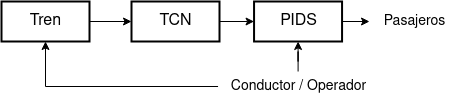
\includegraphics[width=0.66\textwidth]{./Figures/diagTrenTcnPids.png}
	\caption{Diagrama del sistema Tren-TCN-PIDS.}
	\label{fig:diagTrenTcnPids}
\end{figure}

La red TCN define una comunicación estándar usando dos buses jerárquicos llamados WTB(Wire Train Bus) y MVB (Multifunction Vehicle Bus). El sistema PIDS se interconecta al bus de datos MVB, como se indica en el diagrama de la figura \ref{fig:diagTcnPidsBuusesWtbMvb}.\\


\begin{figure}[ht]
	\centering
	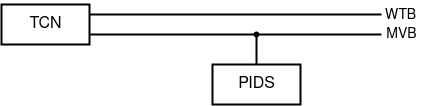
\includegraphics[width=0.66\textwidth]{./Figures/diagTcnPidsBusesWtbMvb.png}
	\caption{Diagrama de interconexión TCN-PIDS}
	\label{fig:diagTcnPidsBuusesWtbMvb}
\end{figure}

El sistema PIDS tiene un bus de comunicación propio a través de una red RS485. Uno de los componentes de esta red es el módulo SCU, al cual se conectan distintos dispositivos como los display LED, los mapas de recorrido LED, las cámaras y parlantes, tal como se indica en la figura 	\ref{fig:diagPidsScuDevices}.\\


\begin{figure}[ht]
	\centering
	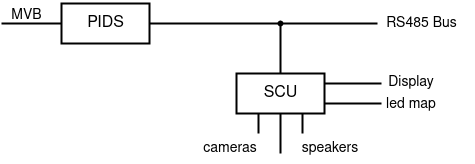
\includegraphics[width=0.66\textwidth]{./Figures/diagPidsScuDevices.png}
	\caption{Diagrama del módulo SCU en la red PIDS.}
	\label{fig:diagPidsScuDevices}
\end{figure}

Al módulo SCU se conectan las unidades IDU, que corresponden a los display LED de salón. Cada unidad IDU contiene un driver y el arreglo de módulos de matriz de led que conforman el display. En la figura \ref{fig:diagScuDriverDisplay} se representan estos bloques funcionales.\\


\begin{figure}[ht]
	\centering
	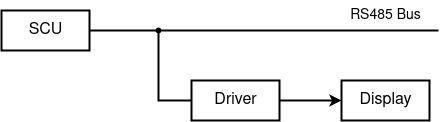
\includegraphics[width=0.66\textwidth]{./Figures/diagScuDriverDisplay.png}
	\caption{Diagrama de bloques del sistema SCU, placa de control y carteles LED de salón.}
	\label{fig:diagScuDriverDisplay}
\end{figure}

El alcance del sistema desarrollado en este trabajo cubre la funcionalidad de este conjunto de bloques Driver + Display, que en la nomenclatura del sistema PIDS existente corresponde a los módulos IDU. Existen dos unidades de estos módulos por cada salón o coche.\\

Comúnmente un tren tiene siete coches en las formaciones de SOFSE, por lo que se tiene un mínimo de catorce unidades IDU más dos displays externos adicionales para el frente y contrafrente del tren que indican las estaciones cabecera del recorrido. Esto resulta en un total de dieciséis unidades de control de display por cada tren. Teniendo en cuenta las formaciones operativas de las líneas Mitre, Sarmiento y Roca del Área Metropolitana de Buenos Aires (AMBA), se puede estimar alrededor de treinta trenes operando en simultáneo, lo que resulta en aproximadamente 500 unidades de displays operando en vivo. El impacto que puede tener el aporte de este trabajo estará directamente relacionado con la operación de Trenes Argentinos y definitivamente puede contribuir a la extensión de la vida útil de los trenes.\\

\subsection{Diseño}
La propuesta de diseño busca cubrir las funcionalidades del bloque de control del display LED. El display LED es una unidad que se puede adquirir comercialmente. Sin embargo el driver para la red PIDS es una solución propietaria del fabricante y es la que se busca reemplazar con este desarrollo.\\

En la figura \ref{fig:diagVistaReDisenhoEduCIAA} se presenta un diagrama de bloques del sistema de control propuesto. Este controlador usa comunicación serie a través de interfaces UART-RS485 y UART-USB. La UART es un periférico del microcontrolador de la plataforma CIAA. La alimentación de la CIAA difiere de aquella existente en la red RS485, por lo que también es necesario un bloque de conversión DC-DC para garantizar compatibilidad eléctrica. La comunicación con el display se realiza a través de un adaptador, que consiste básicamente en un puerto de entrada-salida.\\


\begin{figure}[ht]
	\centering
	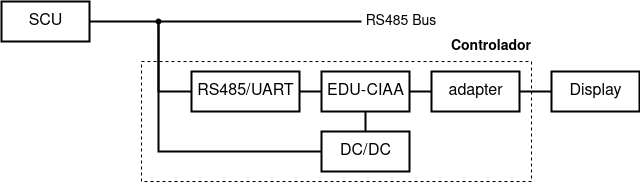
\includegraphics[width=0.75\textwidth]{./Figures/diagVistaReDisenhoEduCIAA.png}
	\caption{Diagrama de bloques del controlador propuesto.}
	\label{fig:diagVistaReDisenhoEduCIAA}
\end{figure}

A nivel lógico, el sistema que se propone consiste en cuatro objetos activos que interactúan entre sí, tal como se indica en la figura \ref{fig:diagVistaDisenho}. 

\begin{figure}[ht]
	\centering
	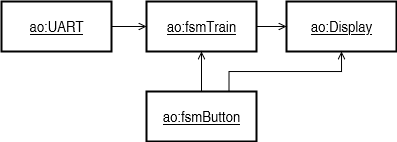
\includegraphics[width=1\textwidth]{./Figures/diagVistaDisenho.png}
	\caption{Vista de interacciones del sistema propuesto.}
	\label{fig:diagVistaDisenho}
\end{figure}

El objeto activo UART es el encargado de recibir e interpretar las tramas de datos que viajan por la red RS485 del bus de datos del SCU. El objeto activo fsmButton es el control manual del operador para accionar el sistema. El objeto activo fsmTrain es una máquina de estados que representa el estado del tren y es el que contiene los mensajes y nombres de las estaciones. El objeto activo Display es el encargado de codificar los mensajes en el formato correspondiente a la matriz led del display.\\

Esta vista de interacción entre objetos indica la dependencia funcional de los componentes del sistema. Su diseño modular permite hacer cambios en los componentes de sistema de forma independiente. Por ejemplo se podrían reemplazar los mensajes al pasajero en el objeto fsmTrain sin afectar el resto del sistema, o bien reemplazar la lógica de control del display si fuera necesario cambiar la tecnología de control del display led modificando únicamente el objeto Display.\\


\section{Implementación}
En este trabajo se implementa un sistema embebido en lenguaje C usando el sistema operativo de tiempo real freeRTOS sobre una arquitectura de 32 bits ARM Cortex-M4/M0. La plataforma de hardware elegida es la CIAA-EDU-NXP, que dispone de un microcontrolador LPC4337 de la companía NXP (\cite{NXPLPC4337}).\\
 
Se ha utilizado la \textit{SAPI} y el \textit{firmwareV3} \cite{firmwarev3}, como API que funciona como capa de abstracción de las funciones específicas de la biblioteca del fabricante del microcontrlador. Esta API es parte fundamental del proyecto CIAA.\\
 
En el desarrollo del firmware se ha preferido el uso de plantillas para implementar patrones de software como máquinas de estado y objetos activos, de manera que se facilite la documentación y testing y con ello el mantenimiento y la escalabilidad. Se describen los lineamientos y fragmentos de código principales en la sección de patrones de software.\\

Finalmente se dedica una sección a nivel de detalle para la implementación del controlador del diplay led. El firmware busca ser portable a aquellas versiones de hardware de display basadas en el conjunto de chips 74HC245, 74HC595 y 74HC138 o equivalentes de compuertas digitales. \\


\subsection{Organización del código fuente}
La organización del código fuente que conforma el sistema embebido de este trabajo se describe en el siguiente árbol de archivos:

\begin{lstlisting}[
	language=Bash, 
	backgroundcolor=\color{mygray},
	]
AppRTOS
|-- config.mk
|-- inc
|   |-- displayLed.h
|   |-- FreeRTOSConfig.h
|   |-- ISR_GPIO.h
|   |-- main.h
|   |-- modulePanelDisplay.h
|   |-- portmap.h
|   |-- statemachine_AB.h
|   |-- statemachine_button.h
|   |-- statemachine_displayLed.h
|   `-- userTasks.h
|-- LICENSE.txt
`-- src
    |-- displayLed.c
    |-- ISR_GPIO.c
    |-- main.c
    |-- statemachine_AB.c
    |-- statemachine_button.c
    |-- statemachine_displayLed.c
    `-- userTasks.c
\end{lstlisting}

Se pueden observar dos directorios principales: \textit{inc} y \textit{src}. En \textit{inc} se incluyen los archivos de encabezados y en \textit{src} los archivos de código ejecutable. Existe un archivo principal o \textit{main} que es el que instancia las secuencias de incialización, recursos y tareas del sistema operativo. Las tareas, entendidas como los objetos activos y procesos del sistema, se implementan en los archivos \textit{userTasks}. Luego, para cada implementación de objeto activo existe una máquina de estados asociada en un archivo de encabezados y un archivo ejecutable con el prefijo \textit{statemachine}. Finalmente los archivos con el prefijo \textit{ISR} corresponden a las rutinas de interrupción.\\

Esta organización permite encapsulamiento y modularidad entre componentes del sistema. Con ello se facilita el mantenimiento y con el uso de las mismas reglas de diseño y plantillas se facilita la escalabilidad.\\

\subsection{RTOS: Sistema operativo de tiempo real}

En este desarrollo se utiliza freeRTOS, una versión en C de un kernel de sistema operativo de tiempo real. La implementación se basa en la inclusión de los archivos FreeRTOS.h y FreeRTOSConfig.h. Esta implementación ha sido validada en arquitecturas ARM Cortex-M4, en particular en la plataforma EDU-CIAA. 

En todos los casos que fue posible se utilizaron semáforos, colas y mutex para organizar y proteger el uso compartido de recursos. \\

El caso de uso típico de \textit{mutex} es la interacción de distintas tareas con la misma interfaz UART-USB para imprimir mensajes por pantalla. En el código fuente de cada objeto implementado se utiliza la siguiente plantilla para proteger el recurso evitando accesos múltiples y posibilidad de deadlock:\\

\begin{lstlisting}[
	language=C, 
	backgroundcolor=\color{mygray},
	]
if (pdTRUE == xSemaphoreTake( xMutexUART, portMAX_DELAY)){
   vPrintString("Task AB is running.\r\n");
   xSemaphoreGive(xMutexUART);
}
\end{lstlisting}

Las colas, \textit{Queue}, se utilizan principalmente para comunicar eventos entre objetos activos. En todos los casos se referencian con handlers usando la nomenclatura con prefijo \textit{queueHandle}. En el siguiente fragmento de código se muestra un ejemplo, exibiendo los mecanismos de control de errores usados. \\

\begin{lstlisting}[
	language=C, 
	backgroundcolor=\color{mygray},
	]
queueHandle_button = xQueueCreate(QUEUE_MAX_LENGTH, sizeof(eSystemEvent_button));
if (queueHandle_button == NULL){
    perror("Error creating queue");
    return 1;
}
\end{lstlisting}


Todas las tareas y recursos del sistema operativo se han protegido contra errores informando al usuario ante fallas en la instanciación previas al inicio del scheduler.

\begin{lstlisting}[
	language=C, 
	backgroundcolor=\color{mygray},
	]
if( xTaskCreate( vTaskReadSerial, "Serial Comm reading task", 
    configMINIMAL_STACK_SIZE*4, NULL, tskIDLE_PRIORITY+2, &xTaskReadSerialHandler) 
    == pdFAIL ) {
    perror("Error creating task");
}
\end{lstlisting}

Se utilizan también punteros de tipo \textit{xTaskHandle}para referenciar las tareas del sistema operativo. Este tipo de referencias es de especial utilidad a la hora de crear o eliminar tareas de forma dinámica en tiempo de ejecución. También es posible usar estas referencias para comunicación interprocesos, o entre tareas.\\

También se utilizan \textit{Timers} por software en aquellos casos que su uso facilita el mantenimiento, legibilidad y comprensión de la implementación. Especial cuidado de superposición o competición del reloj del sistema operativo se procura al disponer de componentes que tienen requisitos temporales que compiten entre si por prioridad del scheduler. Se verá en detalle la implementación del display Led como ejemplo.\\

Finalmente, se han utilizado rutinas de interrupciones o \textit{ISR} en aquellos casos que se requiere respuesta inmediata, como el accionamiento manual de un interruptor o bien la comunicación del bus de datos del tren. El caso de uso de interrupciones se representa en la figura \ref{fig:ISR}.

\begin{figure}[ht]
	\centering
	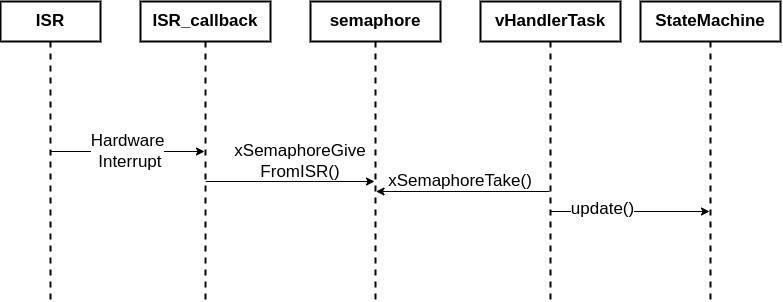
\includegraphics[width=1\textwidth]{./Figures/ISR_semaphore.png}
	\caption{Diagrama de secuencia que representa la interacción entre componentes del sistema operativo cuando se dispara una interrupción o ISR.}
	\label{fig:ISR}
\end{figure}

El recurso de hardware que genera una interrupción (ISR) tiene asignado una función específica \textit{ISR callback} que entrega un semáforo que luego es tomado por una tarea de sistema (vHandlerTask). Esta última normalmente representa un objeto activo que actualiza una máquina de estado.\\

\subsection{Patrones de software}
En este desarrollo se ha hecho uso extensivo de los patrones máquina de estado, objeto activo, pipeline, observ and react, y superciclo. Se presenta en detalle el formato de plantillas desarrollado en C para freeRTOS.\\

\subsubsection{Máquinas de estado}
El desarrollo de la arquitectura orientada a eventos propuesta se basa en la interacción de máquinas de estado usando objetos activos. En este trabajo las máquinas de estado se implementan sistemáticamente en C con el siguiente procedimiento paso a paso:

\begin{enumerate}
\item Representar los estados y eventos con un diagrama de máquina de estados.
\begin{figure}[ht]
	\centering
	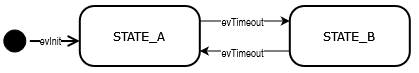
\includegraphics[width=0.66\textwidth]{./Figures/statemachineAB.png}
	\caption{Diagrama de la máquina de estados AB ejemplo.}
	\label{fig:fsmAB}
\end{figure}

\item Definir los estados. Usar tipo enumerativo definido con el prefijo \textit{eSystemState}:

\begin{lstlisting}[
	language=C, 
	backgroundcolor=\color{mygray},
	]
typedef enum{

    STATE_INIT,
	STATE_A,
	STATE_B

} eSystemState;
\end{lstlisting}

\item Definir los eventos. Los eventos representan transiciones entre estados con un tipo definido con el prefijo \textit{eSystemEvent}:

\begin{lstlisting}[
	language=C, 
	backgroundcolor=\color{mygray},
	]
typedef enum{

	evInit,
	evTimeout

} eSystemEvent;
\end{lstlisting}

\item Definir un tipo puntero a función para designar los handlers con el prefijo \textit{*pfEventHandler()}:

\begin{lstlisting}[
	language=C, 
	backgroundcolor=\color{mygray},
	]
typedef eSystemState (*pfEventHandler)(void);
\end{lstlisting}

\item Definir una estructura para la máquina de estados con un tipo \textit{sStateMachine}. Esta estructura debe incluir una variable estado (eSystemState), una variable evento (eSystemEvent) y un puntero a función (pfEventHandler). El puntero a función será una instancia de handler específico que maneje las transiciones entre estados. 

\begin{lstlisting}[
	language=C, 
	backgroundcolor=\color{mygray},
	]
typedef struct{

	eSystemState  	fsmState;
	eSystemEvent  	fsmEvent;
	pfEventHandler	fsmHandler;

} sStateMachine;
\end{lstlisting}

\item Definir los handlers a implementar para el manejo de ejecución y transiciones entre estados.

\begin{lstlisting}[
	language=C, 
	backgroundcolor=\color{mygray},
	]
eSystemState 	InitHandler(void);
eSystemState 	AtoBHandler(void);
eSystemState 	BtoAHandler(void);
\end{lstlisting}

\item Instanciar la máquina de estados como un arreglo de estructuras de tipo \textit{sStateMachine}. Para el ejemplo de la máquina AB la instancia de arreglo de estructuras sería la siguiente:

\begin{lstlisting}[
	language=C, 
	backgroundcolor=\color{mygray},
	]
sStateMachine_AB fsmMachineAB [] = 
{
	{STATE_INIT_AB, evInit_AB, InitHandler_AB},
	{STATE_A, evTimeout_A, AtoBHandler},
	{STATE_B, evTimeout_B, BtoAHandler}
};
\end{lstlisting}

\item Escribir el código ejecutable de los handlers. Una implementación de handler a modo de ejemplo se presenta a continuación.

\begin{lstlisting}[
	language=C, 
	backgroundcolor=\color{mygray},
	]
eSystemState 	InitHandler(void){ 
	printf("State Machine Init...\n");
	return STATE_A; 
}
\end{lstlisting}

\end{enumerate}

De esta manera queda desacoplada la implentación de los handlers del resto de la estructura de la máquina de estados, logrando portabilidad, escala y modularidad. Los handlers serán funciones que se implementan con el sufijo Handler() y que por definición tienen un solo argumento de tipo void.

Con esta técnica de desacoplamiento, se implementan dos archivos por cada máquina de estado : uno de encabezados (stateMachine.h) con las definiciones y otro con la implementación (stateMachine.c) de los handlers.




\subsubsection{Objeto Activo}
	
Los objetos activos se implementan en esta aplicación como tareas de freeRTOS con dos superciclos anidados de tipo \textit{while(true)}, como se muestra en el siguiente fragmento de código: 

\begin{lstlisting}[
	language=C, 
	backgroundcolor=\color{mygray},
	]
void vTaskAB(void *xTimerHandle)
{
   (void)xTimerHandle;

   // Task successful creation message
   if (pdTRUE == xSemaphoreTake( xMutexUART, portMAX_DELAY)){
      printf("Task AB is running.\r\n");
      xSemaphoreGive(xMutexUART);
   }

   while(true){
      
      // State machine init
      eSystemEvent_AB newEvent	=	evInit_AB;
      eSystemState_AB nextState	=	STATE_INIT_AB;
      fsmMachineAB[nextState].fsmEvent = newEvent; 
      nextState = (*fsmMachineAB[nextState].fsmHandler)();

      // Active object
      while(true){
        if( pdPASS == xQueueReceive(queueHandle_AB, &newEvent, portMAX_DELAY)){
            fsmMachineAB[nextState].fsmEvent = newEvent; 
            nextState = (*fsmMachineAB[nextState].fsmHandler)();
         }
      }
   }
}
\end{lstlisting}

Notar que el primer ciclo while() es el que corresponde al funcionamiento normal de una tarea o proceso de RTOS. En este caso es el encargado de inicializar la máquina de estados asociada al objeto activo. El superciclo while() de la línea 20 se encarga de bloquear la tarea hasta que se reciba un evento por la interfaz (cola de eventos). La interfaz del objeto activo es una cola FIFO con la función de sistema xQueueReceive() (línea 21). Si se recibe un evento, entonces se actualiza el estado de la máquina instanciando el handler que corresponda, como se observa en la línea 25. El diagrama de la figura \ref{fig:AOfsmAB} representa el objeto activo detallado. 

\begin{figure}[ht]
	\centering
	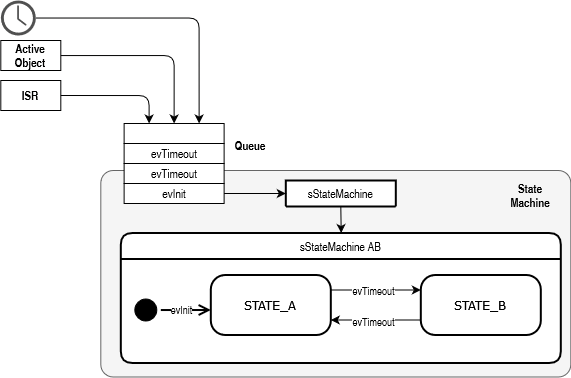
\includegraphics[width=0.85\textwidth]{./Figures/AOstatemachineAB.png}
	\caption{Diagrama del objeto activo de la máquina de estados AB ejemplo.}
	\label{fig:AOfsmAB}
\end{figure}

En este caso la tarea recibe una referencia a un timer (\textit{xTimerHandle}) que genera eventos de timeout y los encola en la interfaz del objeto activo. Con la misma interfaz, los eventos podrían ser generados también por otros objetos activos o por rutinas de interrupción, tal como se indica en la figura.\\




\pagebreak
\subsection{Componentes}


\begin{figure}[ht]
	\centering
	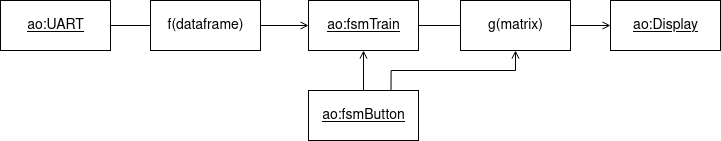
\includegraphics[width=1\textwidth]{./Figures/diagVistaDisenhoExtendida.png}
	\caption{Vista de interacciones extendida del sistema propuesto.}
	\label{fig:diagVistaDisenhoExtendida}
\end{figure}

\begin{figure}[ht]
	\centering
	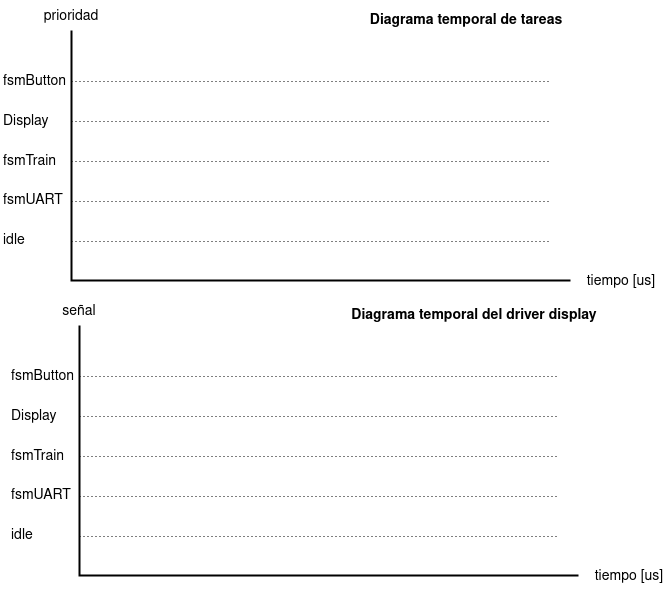
\includegraphics[width=1\textwidth]{./Figures/diagramasTemporales.png}
	\caption{}
	\label{fig:diagramasTemporales}
\end{figure}

\pagebreak
\subsubsection{Display LED}


\begin{figure}[ht]
	\centering
	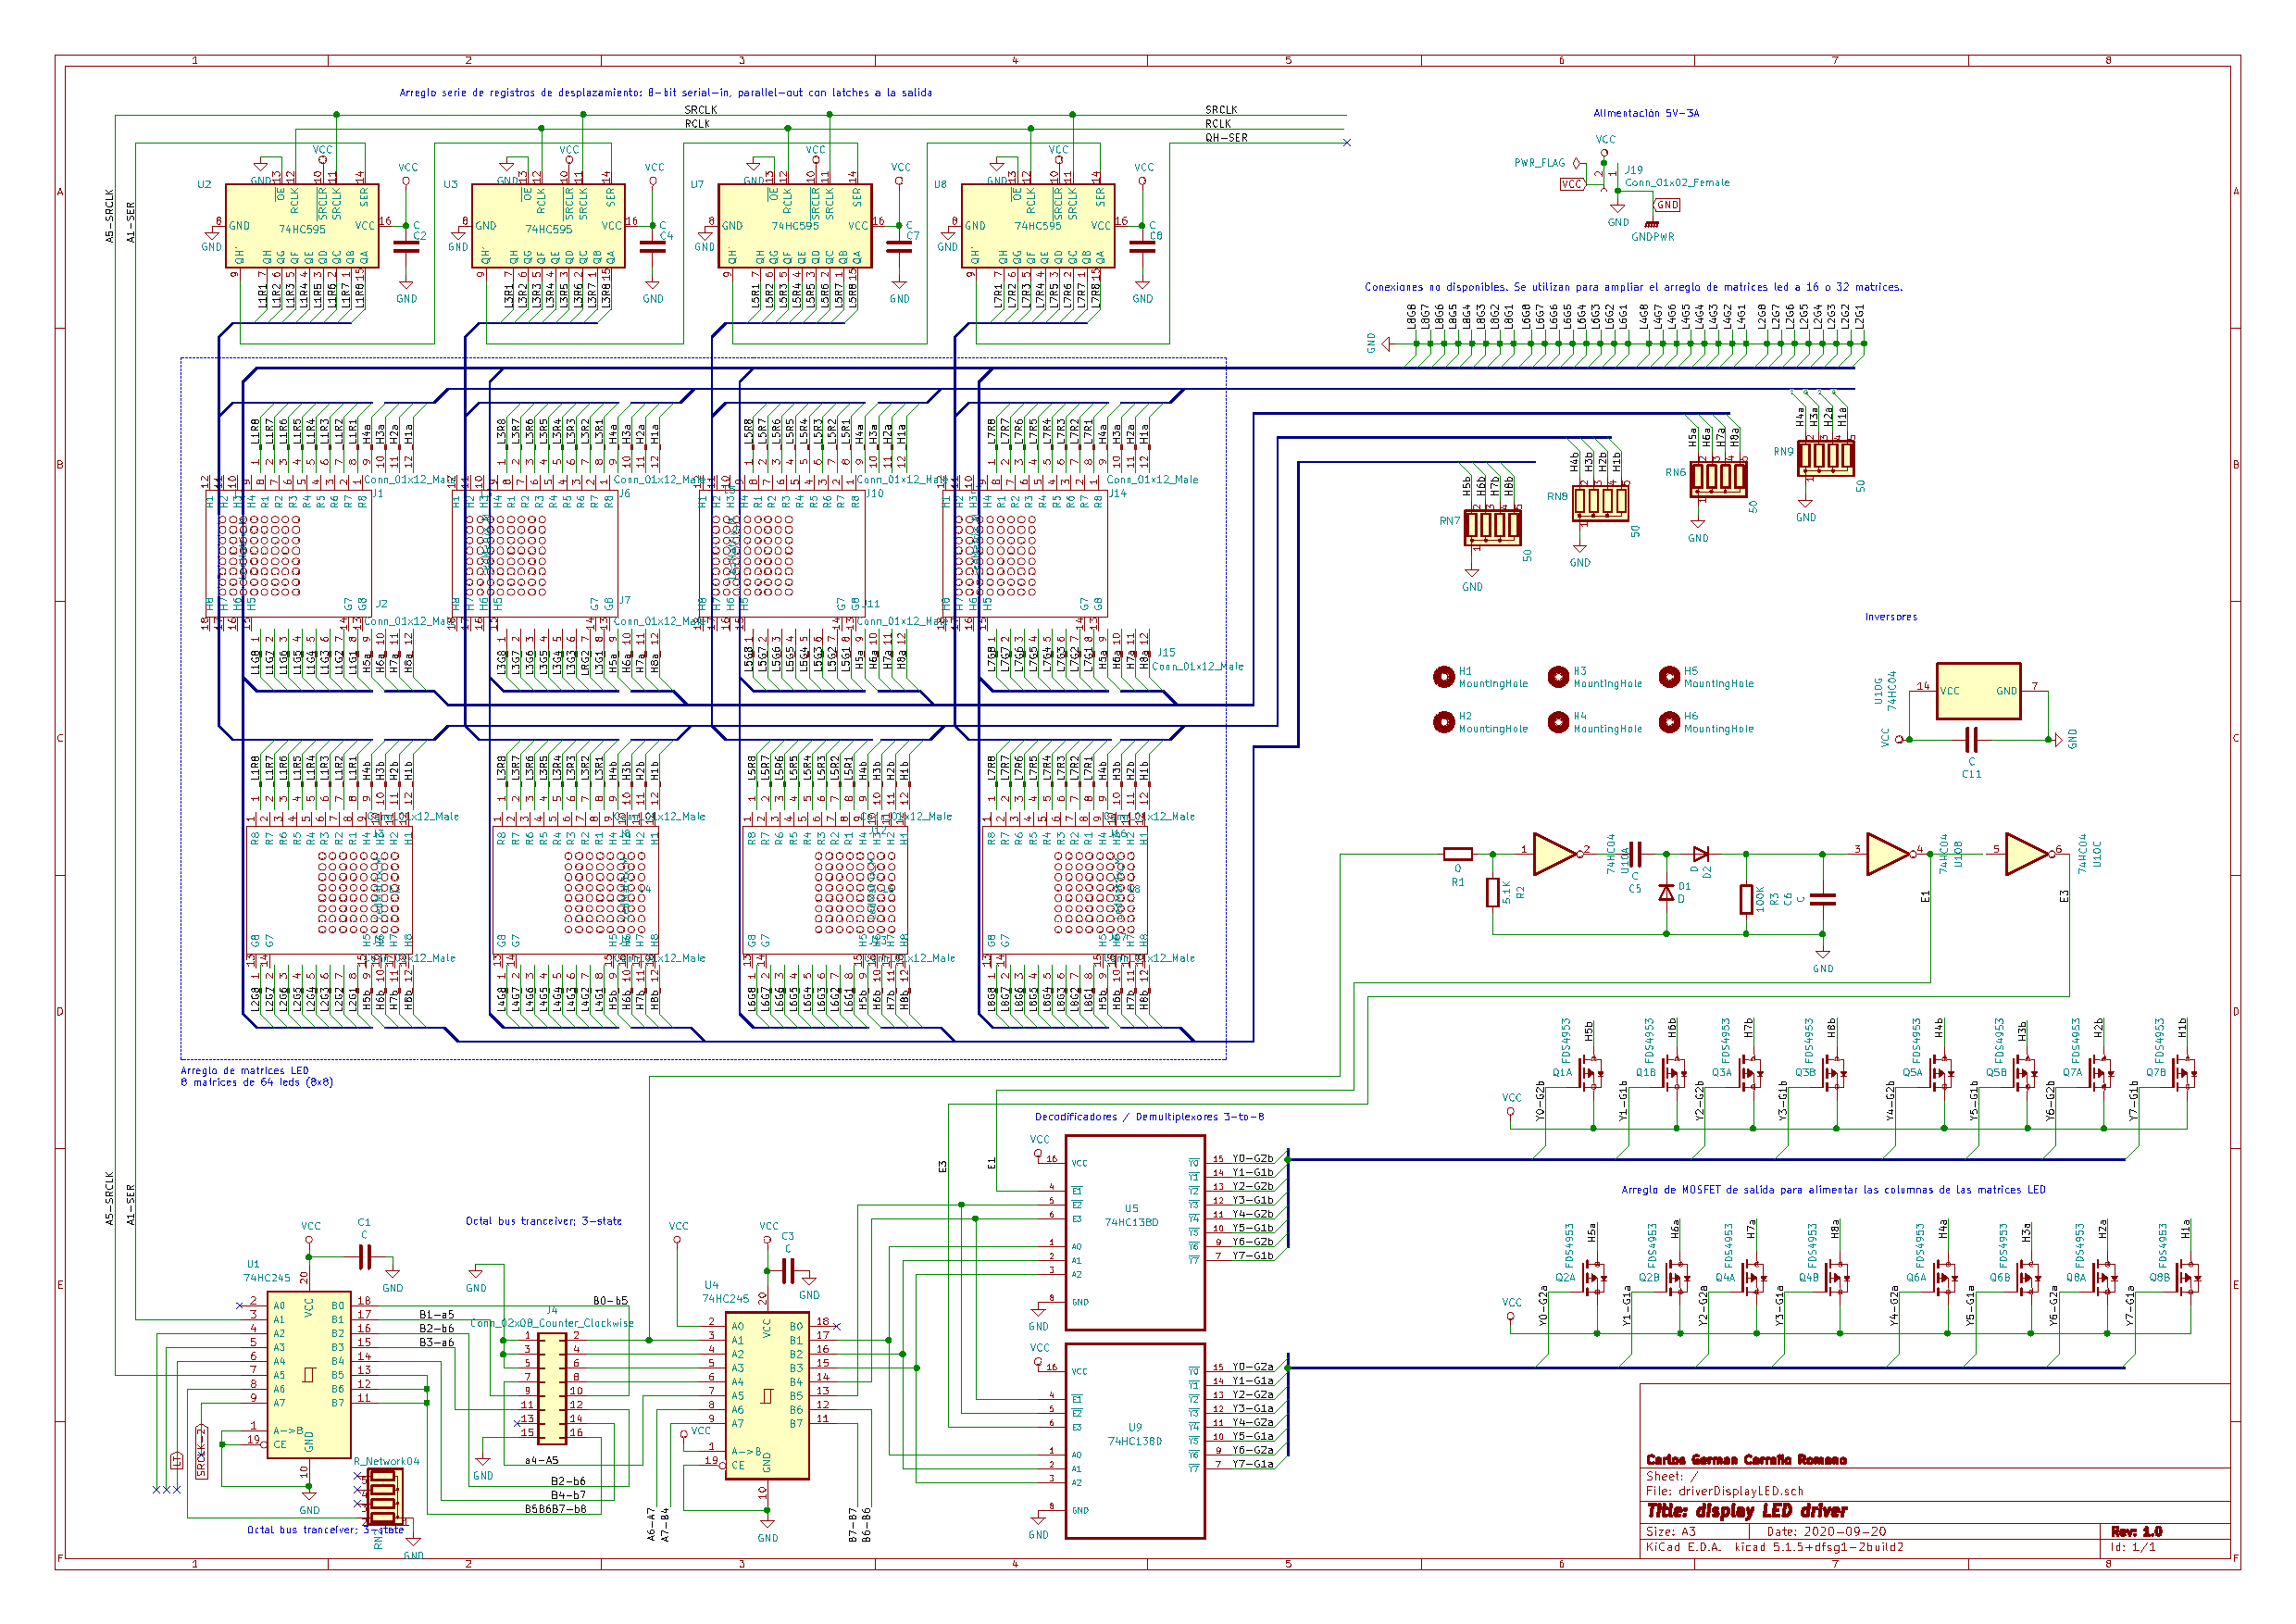
\includegraphics[width=1\textwidth]{./Figures/output.driverLED.pdf}
	\caption{Circuito esquemático de la placa driver de los carteles de matriz LED.}
	\label{fig:schDriverLED}
\end{figure}

\begin{figure}[ht]
	\centering
	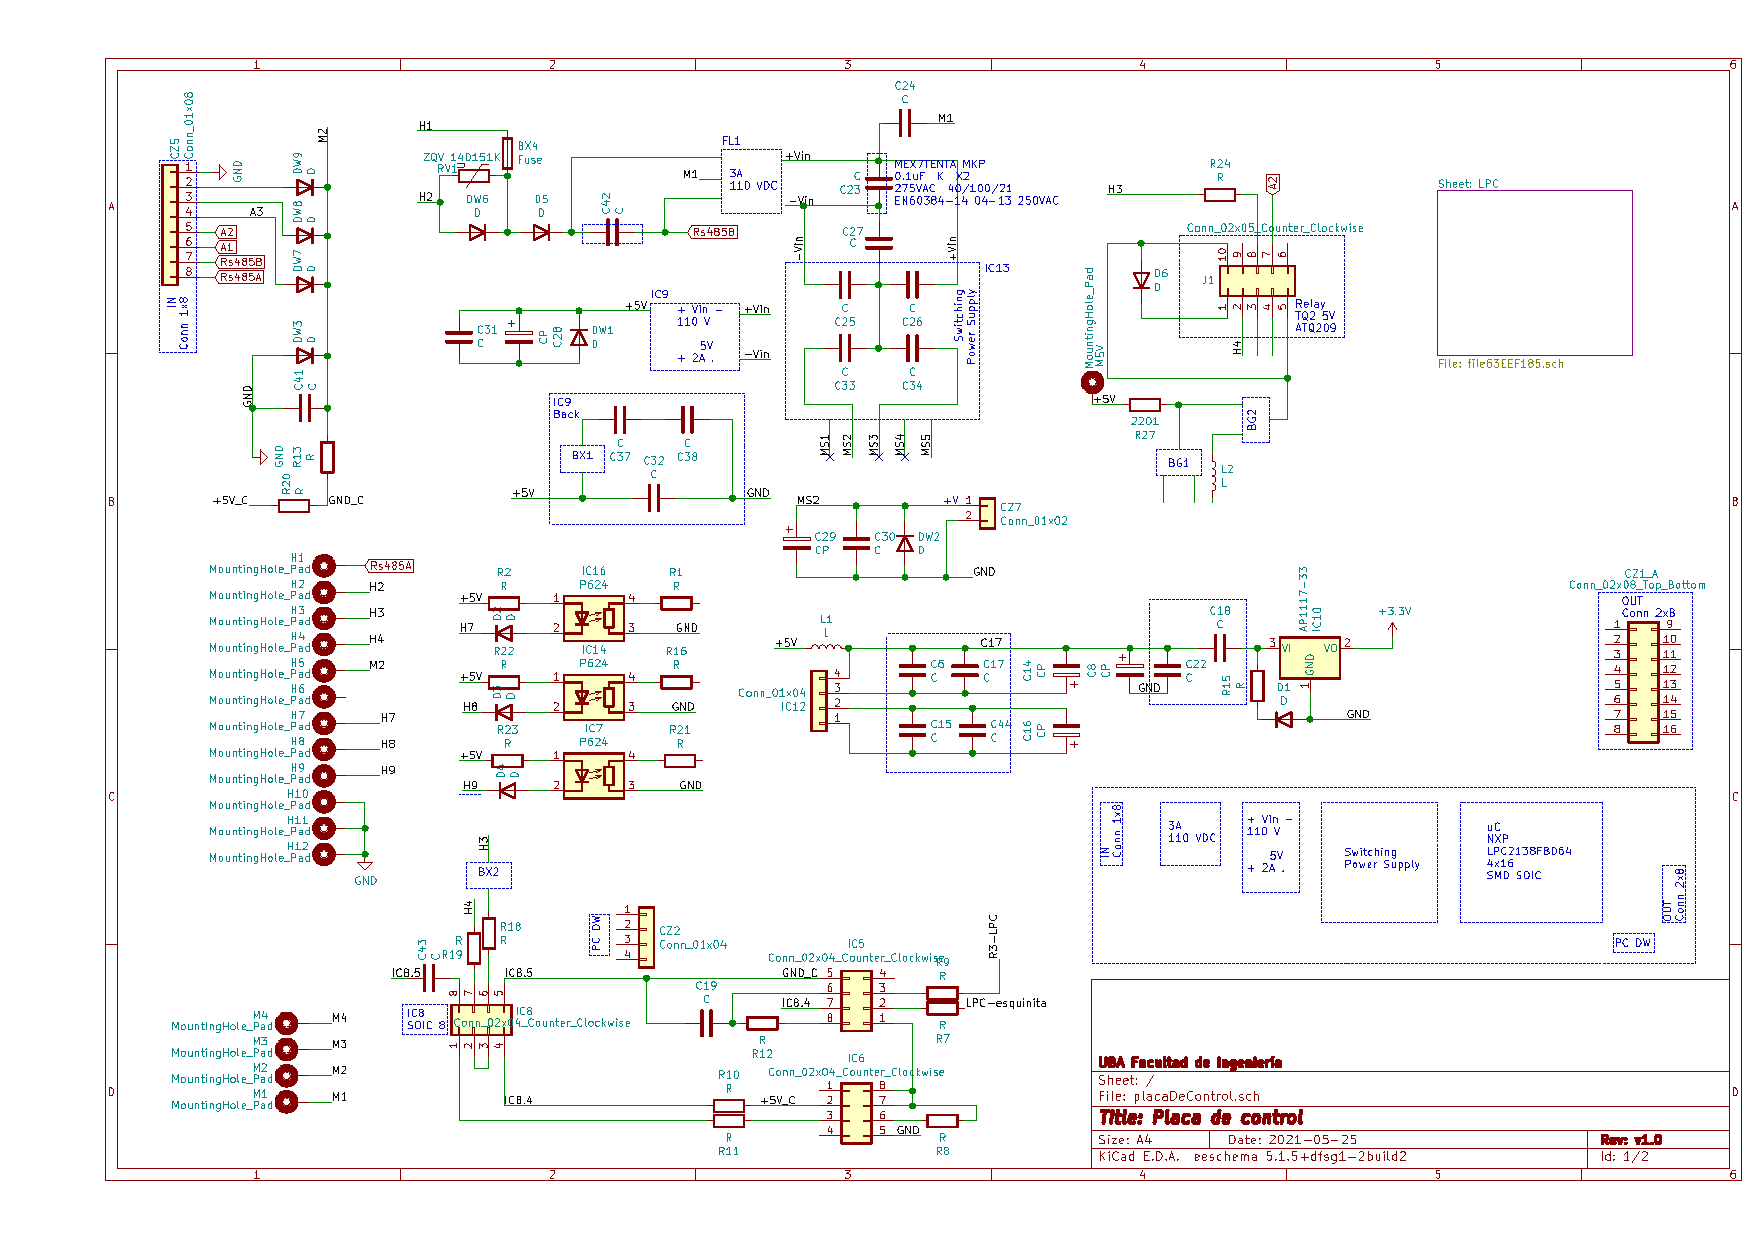
\includegraphics[width=1\textwidth]{./Figures/output.placaControl.pdf}
	\caption{Circuito esquemático de la placa de control de los carteles LED de salón.}
	\label{fig:schController}
\end{figure}

\begin{figure}[ht]
	\centering
	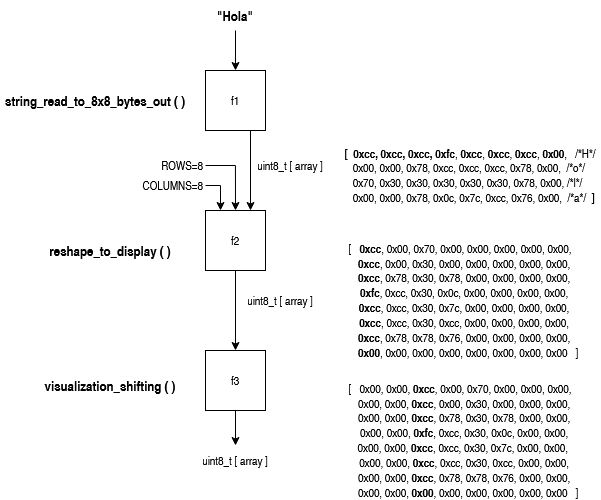
\includegraphics[width=1\textwidth]{./Figures/displayDataLogic.png}
	\caption{Lógica de procesamiento de datos para visualizar en el display.}
	\label{fig:displayDataLogic}
\end{figure}
\subsubsection{Controlador}
\pagebreak
\subsection{Interfaces}
\subsection{Vistas de sistema}

% Chapter Template

\chapter{Ensayos y resultados} % Main chapter title
En este capítulo se detallan los ensayos realizados en las formaciones ferroviarias y en los talleres de Trenes Argentinos. El orden cronológico de los ensayos es distinto al del desarrollo del firmware. En este documento se ha presentado previamente el diseño de la solución para facilitar la comprensión del trabajo realizado. El desarrollo de la solución fue posterior a una serie de mediciones realizadas en los talleres que permitieron identificar parámetros clave del sistema. \\

En las secciones que siguen se explican las mediciones realizadas en las visitas a los talleres de Victoria y Castelar de Trenes Argentinos Operaciones. Luego se presenta un análisis de datos de las tramas relevadas y también las pruebas de integración propuestas para validar el desarrollo. \\


\label{Chapter4} % Change X to a consecutive number; for referencing this chapter elsewhere, use \ref{ChapterX}

%----------------------------------------------------------------------------------------
%	SECTION 1
%----------------------------------------------------------------------------------------

\section{Mediciones}

\section{Análisis de tramas}

\section{Pruebas en maqueta}

En el circuito esquemático de la figura \ref{fig:schDriverled} se presenta el detalle de conexiones eléctricas entre bloques. Se puede observar que a la salida del conector de datos (CONN 2x8) hay dos buffers de la serie 74HC245D que direccionan las señales eléctricas a izquierda y derecha del arreglo de matrices led. A izquierda viajan las señales SER(data), SRCLK (Clock) y XXX (latch) al arreglo de Shift Registers de la serie 74HC595. Por la derecha se maneja la habilitación secuencial de las filas a través de un arreglo de decodificadores 3x8 de la serie 74HC138. Cada salida de los decodificadores se conecta a un driver de corriente en arreglo de transistores MOSFET FDS4953. Estos decodificadores cableados adecuadamente permiten manejar las 32 señales de un cartel de 4x8 módulos led. \\
%
%
%\begin{figure}[ht]
%	\centering
%	%\includepdf[pages={1}, angle=90]{./Figures/output.driverled.pdf}
%	\includegraphics[width=1.66\textwidth, angle=90]{./Figures/output.driverled.pdf}
%	\caption{Circuito esquemático de la placa controladora de los carteles de matriz led.}
%	\label{fig:schDriverled}
%\end{figure}


\begin{figure}[ht]
	\centering
	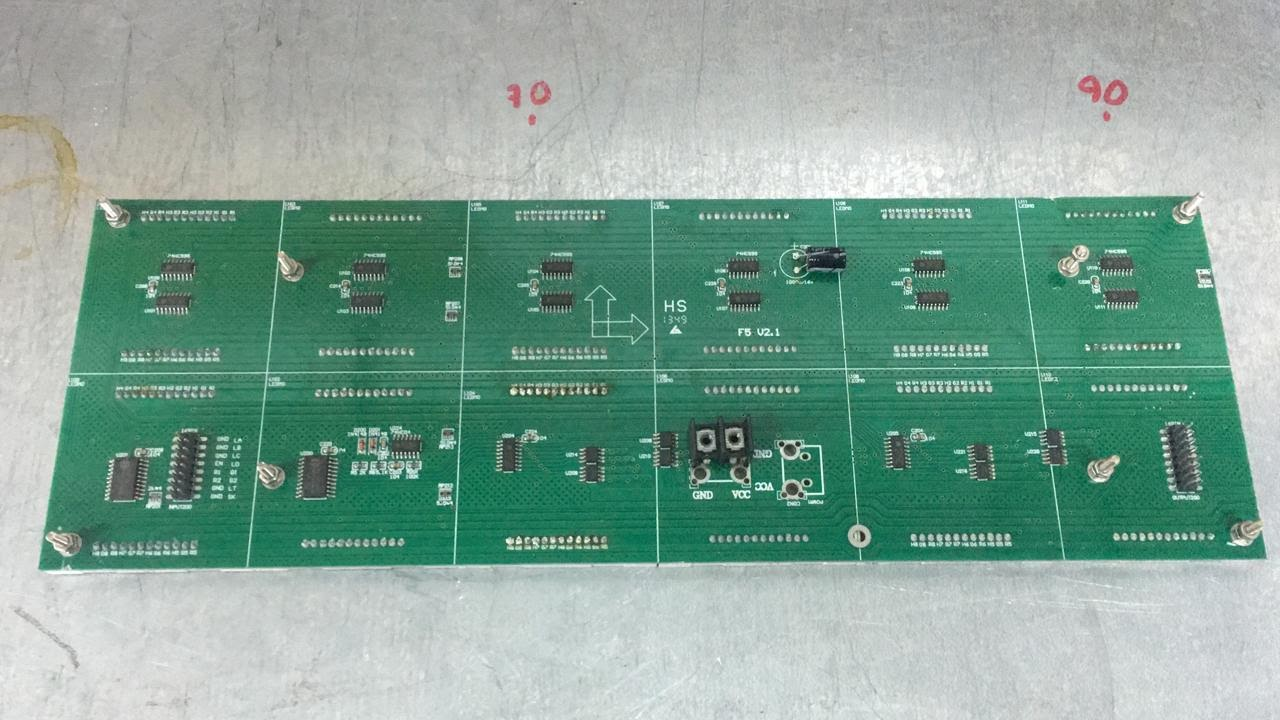
\includegraphics[width=1\textwidth]{./Figures/cartel2x6.jpeg}
	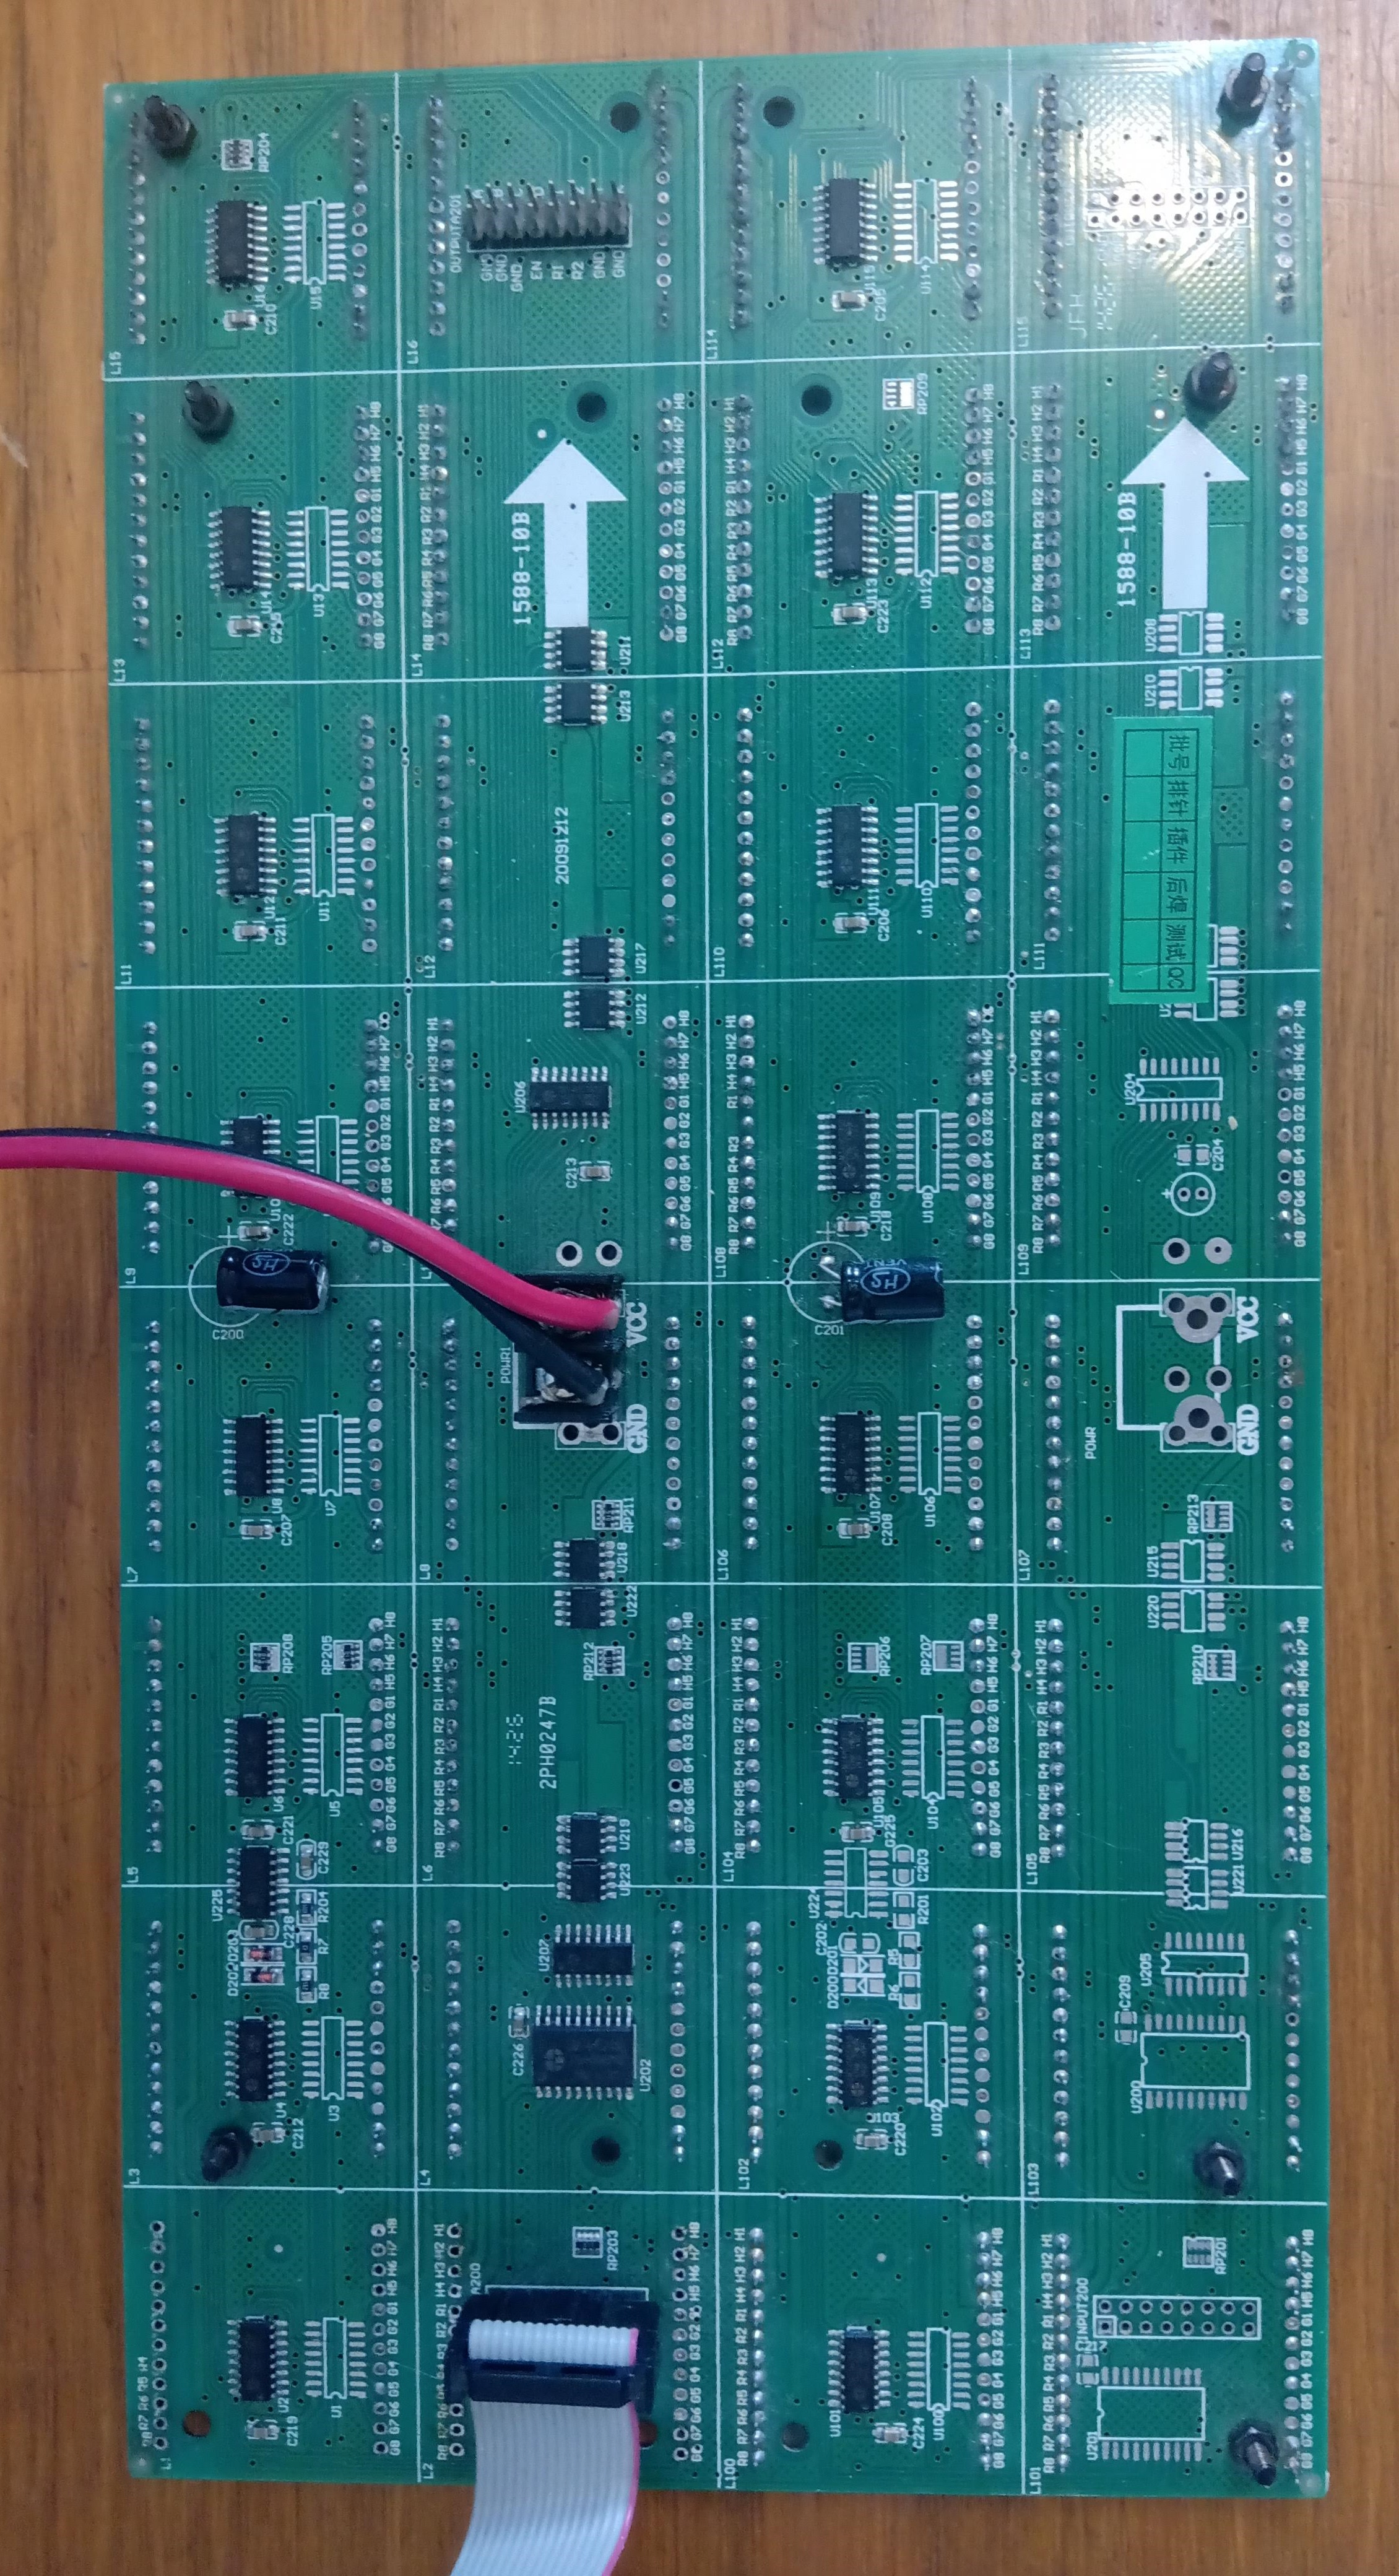
\includegraphics[width=0.75\textwidth, angle=270]{./Figures/cartel4x8.jpg}\\
	\includegraphics[width=1\textwidth]{./Figures/cartelledON.jpg}\\
	\caption{Fotografías de placas de control de los carteles de matriz led: (a) placa de 2x6 módulos; (b) placa de 4x8 módulos; (c) vista posterior de la placa de 4x8.}
	\label{fig:picsDriverled}
\end{figure}


\subsubsection{Placa de control}

\begin{figure}[ht]
	\centering
	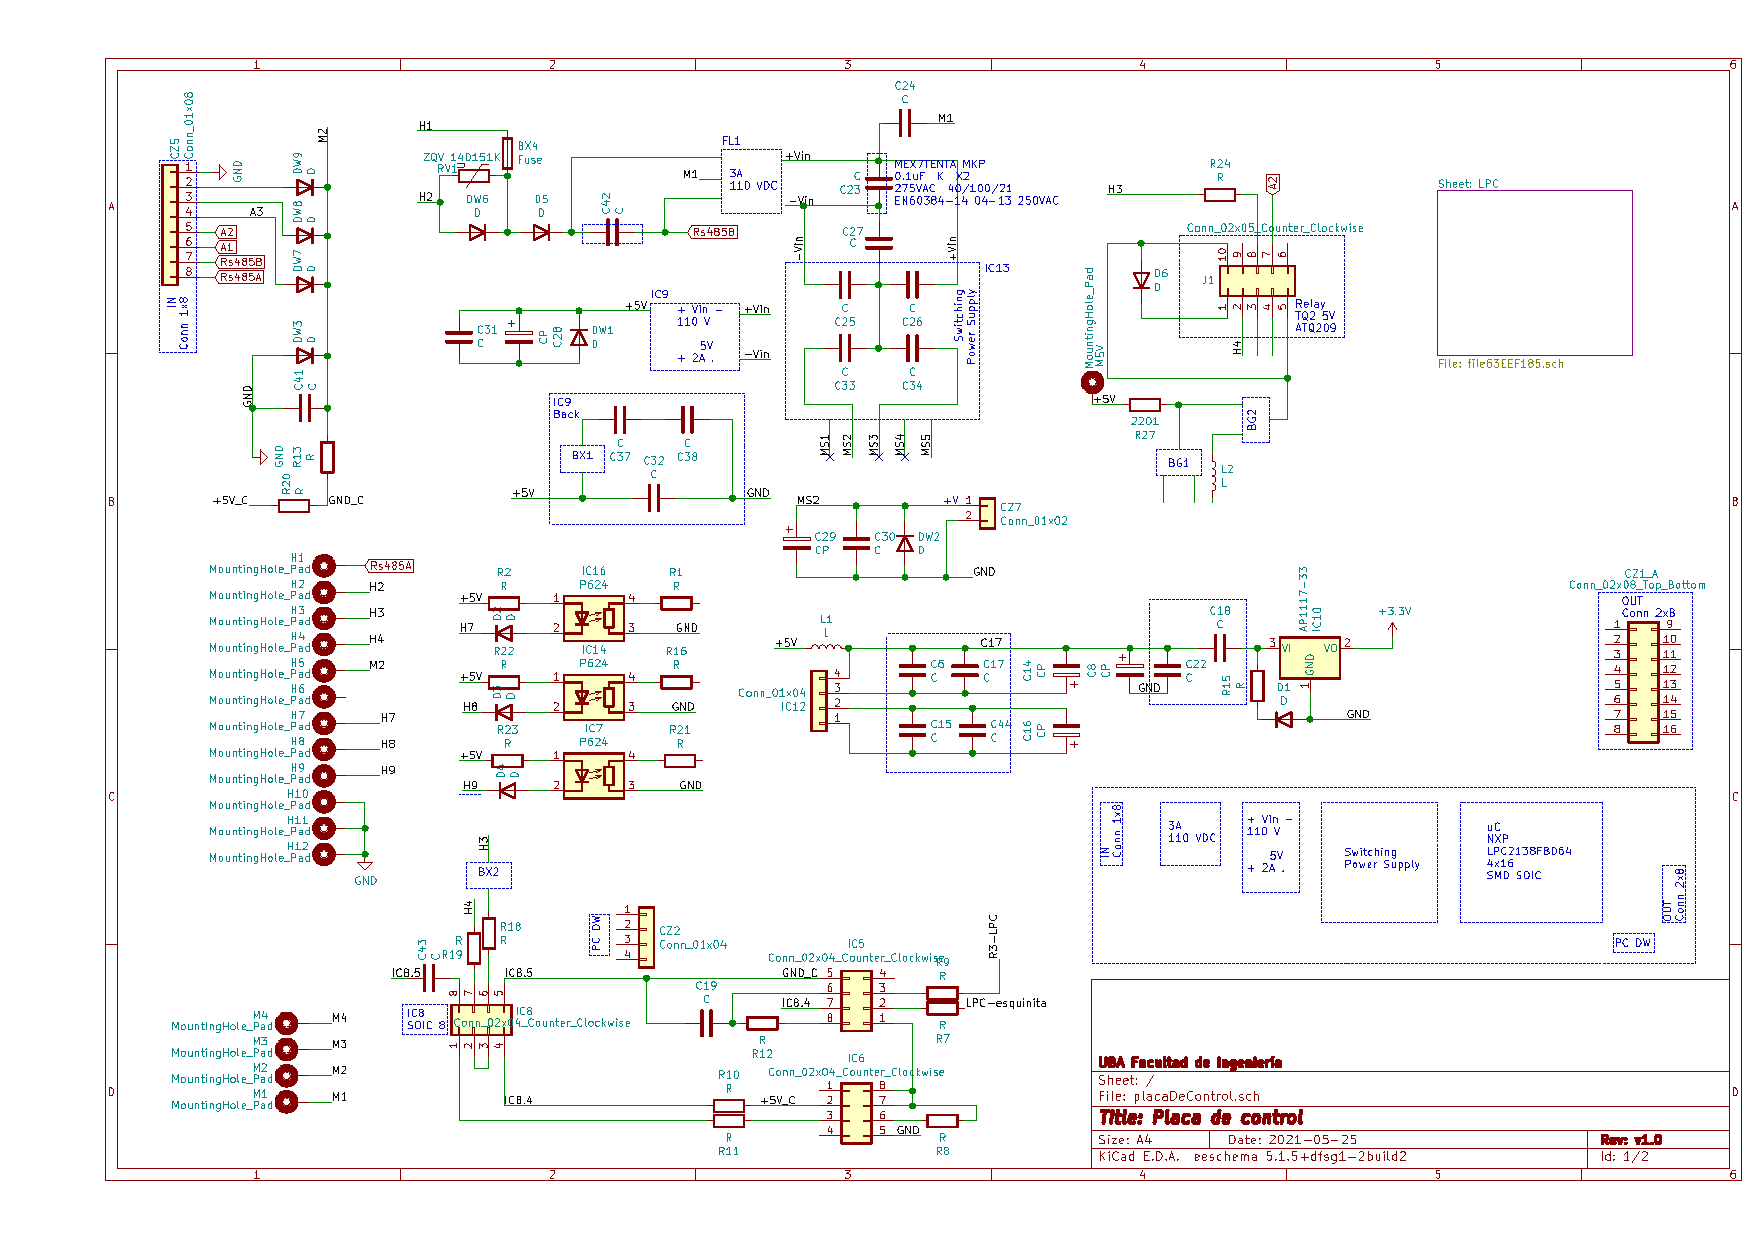
\includegraphics[width=1\textwidth]{./Figures/output.placaControl.pdf}
	\caption{Circuito esquemático de la placa de control de los carteles LED de salón.}
	\label{fig:schController}
\end{figure}


\begin{figure}[ht]
	\centering
	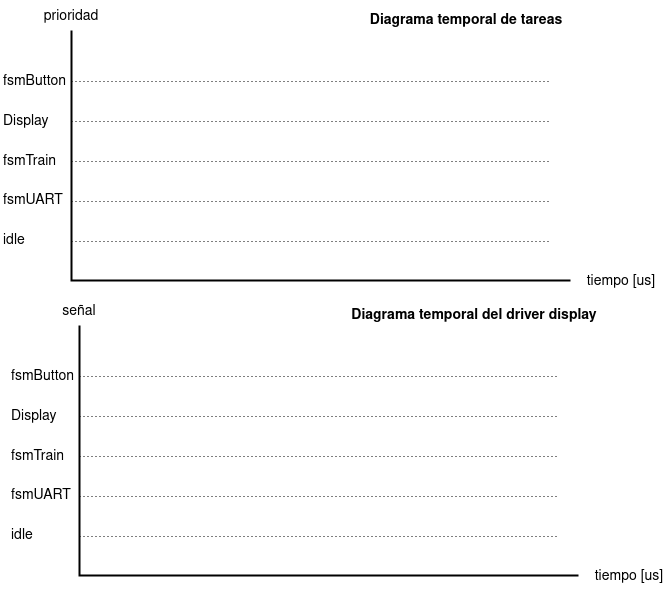
\includegraphics[width=0.5\textwidth]{./Figures/diagramasTemporales.png}
	\caption{}
	\label{fig:diagramasTemporales}
\end{figure}

\section{Integración con red PIDS}

\section{Pruebas de campo}

\begin{figure}[ht]
	\centering
	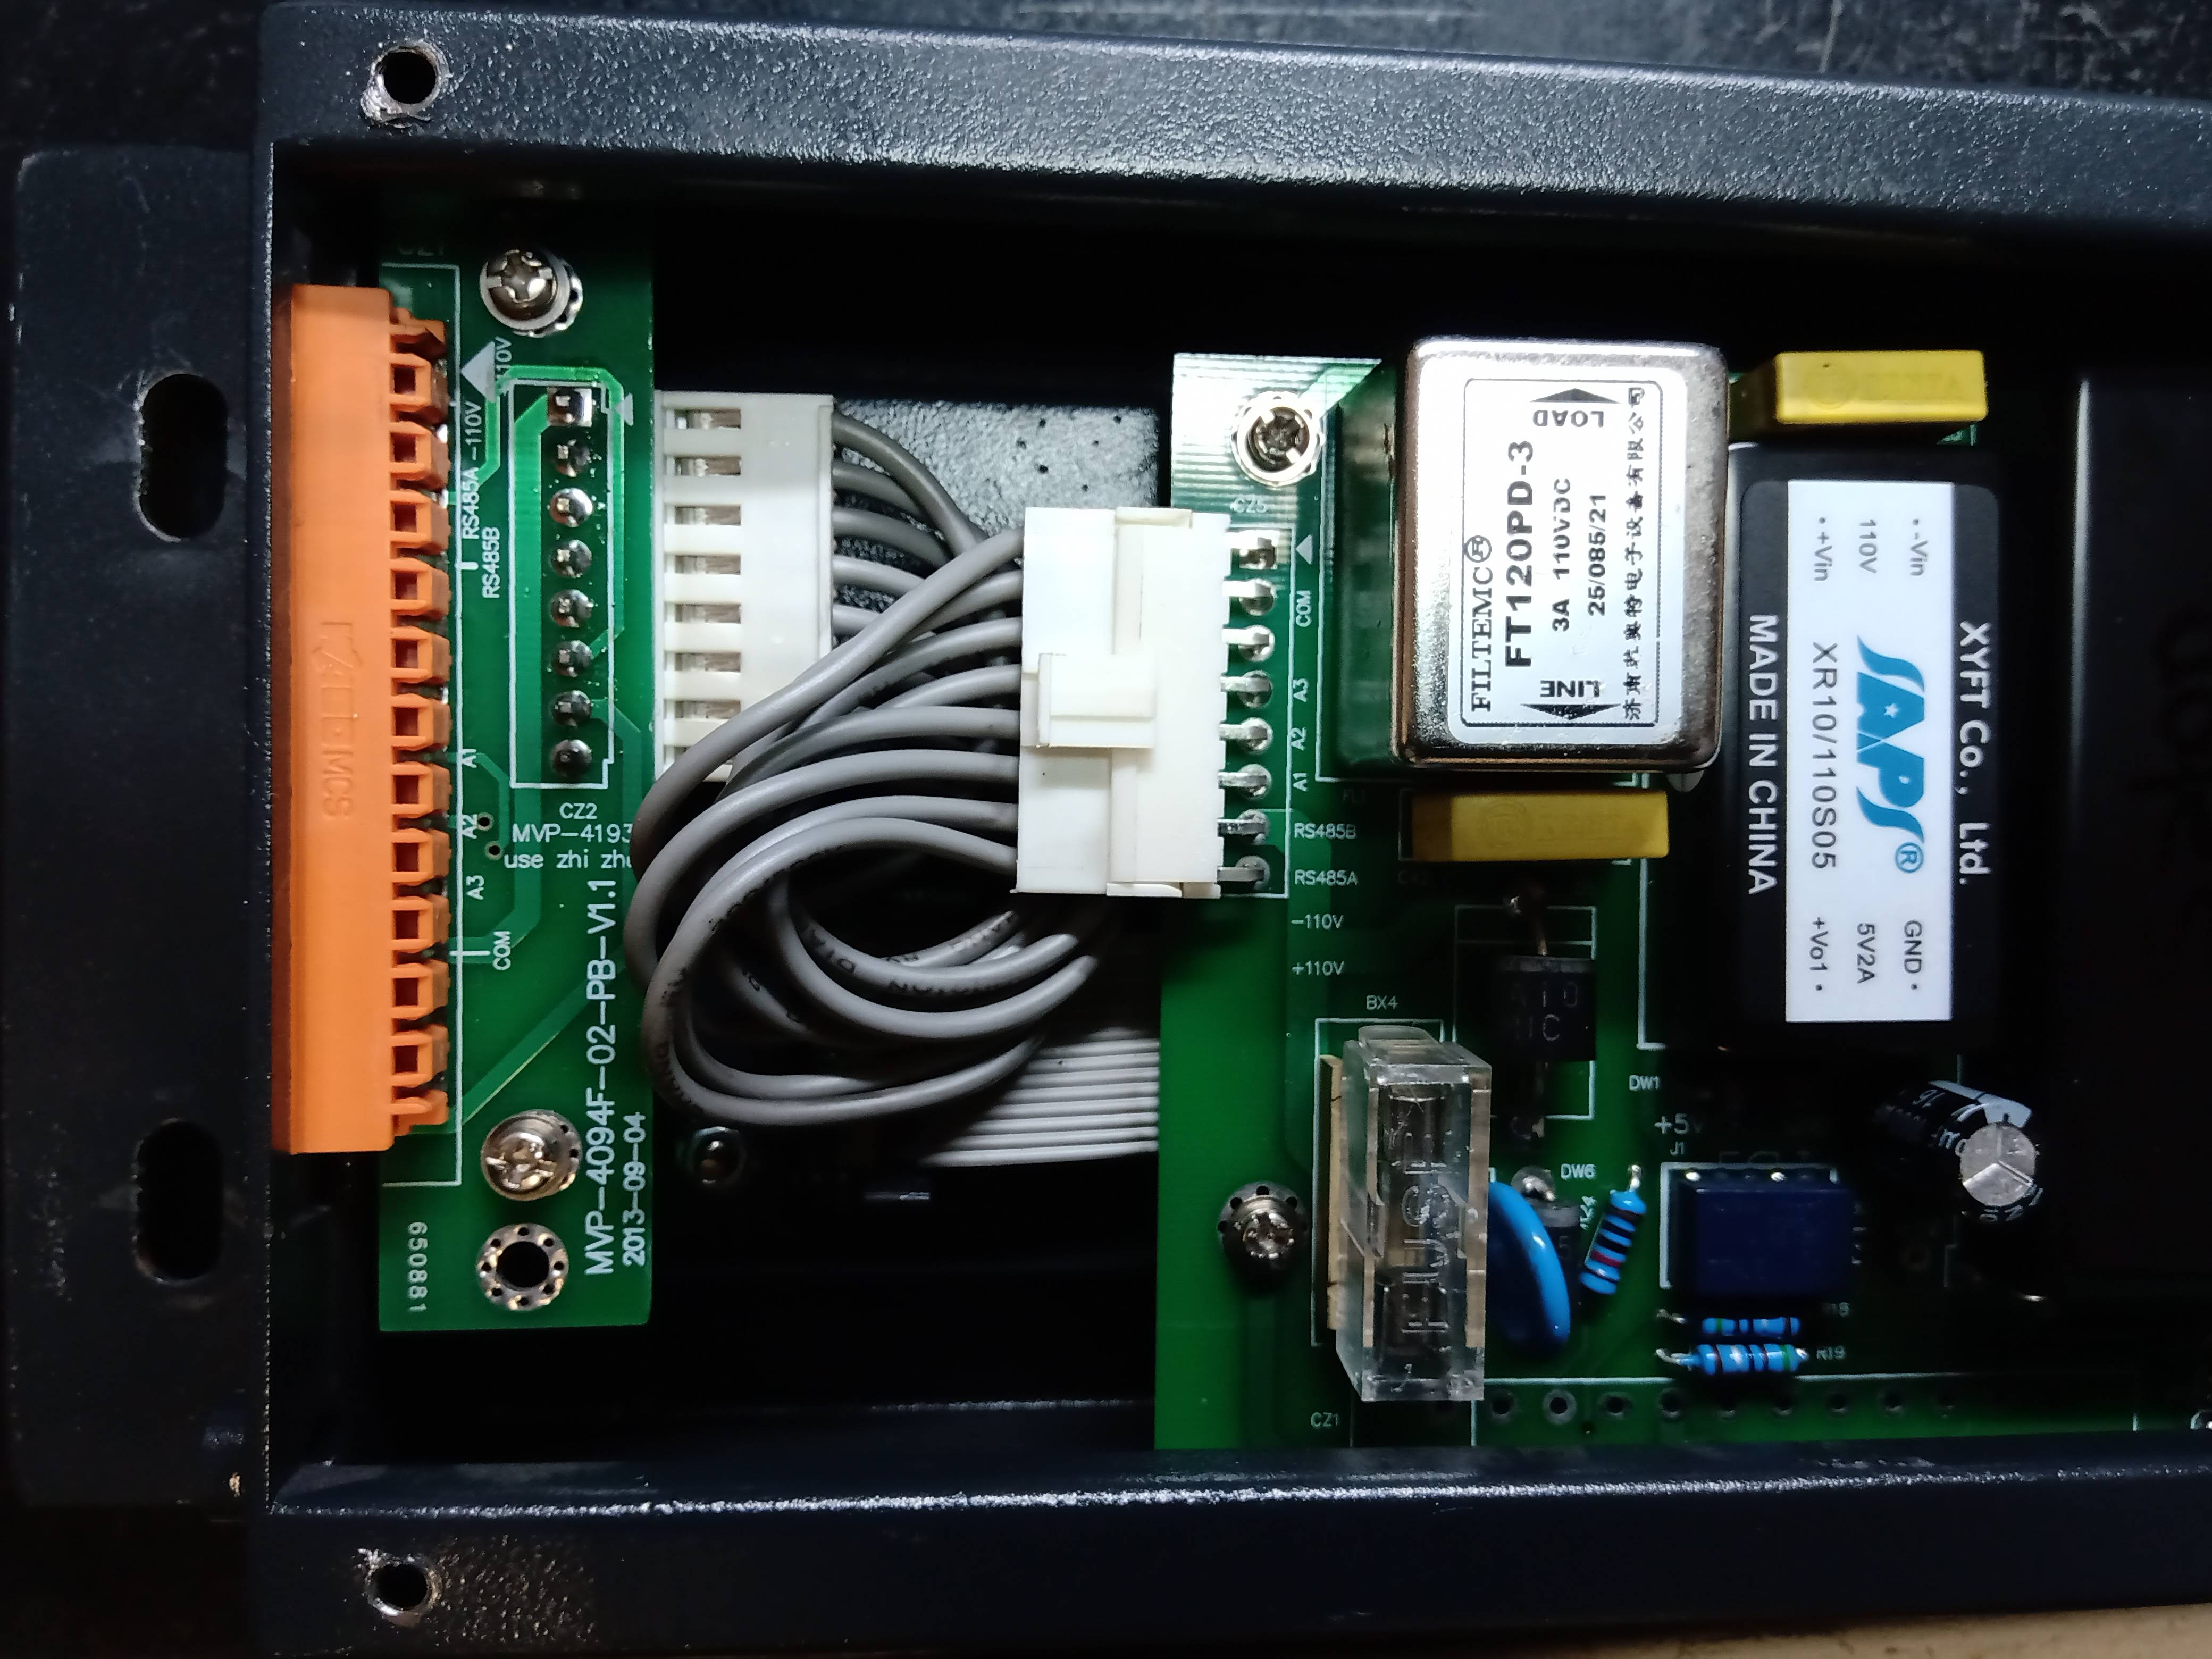
\includegraphics[width=1\textwidth]{./Figures/displayController.jpg}
	\caption{Fotografía del detalle de conexión de la placa de control de los carteles led de salón.}
	\label{fig:displayController}
\end{figure} 
% Chapter Template

\chapter{Conclusiones} % 

En este trabajo se abordó un problema tecnológico de la industria ferroviaria argentina, se desarrolló un sistema embebido, y se realizaron ensayos en las instalaciones de Trenes Argentinos (SOFSE) que aportaron información muy importante para el desarrollo del sistema.\\

La problemática de Trenes Argentinos expuesta en este trabajo, está asociada al mantenimiento del sistema de visualización de información al pasajero (PIDS). Este sistema presenta carteles de matriz led en los coches, y forma parte de un sistema de red más grande que se encarga de las comunicaciones del tren (TCN). La red TCN está ampliamente utilizada en el transporte ferroviario mundial, y los estándares internacionales que la especifican tienen un rol clave en la industria. Si bien los protocolos y componentes de la red TCN están definidos en las normas o especificaciones, el sistema PIDS no está incluido en el estándar de la versión de red instalada en los trenes de SOFSE, siendo una solución propietaria de un fabricante con escasa documentación disponible. Esto motivó la realización de una serie de ensayos en las formaciones ferroviarias operativas, y en las maquetas de los talleres de SOFSE, para relevar aspectos técnicos de su implementación aplicando técnicas de ingeniería inversa.\\

A lo largo del trabajo, se expuso la arquitectura del sistema PIDS existente y su relación con la red TCN. En la solución instalada en los trenes, hay una relación física directa entre algunos de los bloques de la arquitectura y el hardware, que fue relevada durante los ensayos. Por el contrario, algunas de las interconexiones de la arquitectura son únicamente a nivel lógico. Se observaron bloques como el SCU o la PCU, que funcionan como concentradores y procesadores de buses de datos, sin tener un módulo único de hardware asociado, sino una serie de equipos funcionando en conjunto en distintas unidades de rack.  Con la información de las interconexiones, se ensayaron mediciones en distintos puntos de prueba: entre el TCMS y el PIDS por ejemplo, entre PCU y SCU, o entre el SCU y el IDU. \\

El análisis de datos de las mediciones, en particular para los puntos de prueba TCMS-PIDS, presentó consistencia para los encabezados y final de trama con la documentación de TCN disponible. Sin embargo, se observó que el comienzo y final de trama era distinto del anterior para el punto de prueba SCU-IDU, donde el IDU corresponde al hardware de control de los carteles de matriz led. Estas observaciones resultaron compatibles con mediciones realizadas por el personal de SOFSE con anterioridad. Si bien esta información fue suficiente para desarrollar los requerimientos, se ha observado también que las tramas contienen información adicional de otros bloques del sistema, aparte de los carteles de matriz led. Aunque no quede claro el contenido completo de las tramas, es decir, todos los bits que forman parte de la carga útil de las tramas recibidas o transmitidas por los módulos IDU, las hipótesis propuestas para el desarrollo del sistema embebido son compatibles con el comportamiento observado.\\


El desarrollo del sistema embebido ha permitido proponer una solución que otorga cierto grado de abstracción y versatilidad para la interpretación de tramas de datos de la red PIDS. El sistema está diseñado para recibir tramas de longitud variable, que representan eventos, a través de un periférico UART usando técnicas de memoria dinámica. Los datos recibidos pueden ser validados y procesados para activar visualizaciones en carteles de matriz led, compatibles con los que hay instalados en los trenes. El mecanismo de visualización de mensajes para los carteles de matriz led, está desacoplado de la recepción y el procesamiento de las tramas. Es decir, por un lado el sistema puede recibir y reaccionar a eventos externos, y por otro puede generar visualizaciones de mensajes precargados, como por ejemplo el nombre de una estación.\\

 En el diseño se abordaron cuestiones de concurrencia, implementando una arquitectura orientadad a eventos. Se desarrollaron módulos que interactúan entre sí de forma dinámica y que responden a eventos asincrónicos, como por ejemplo la recepción de datos vía UART. Así, un objeto recibe un mensaje, otro lo procesa, y otro genera la visualización en el cartel de matriz led. Cada módulo fue implementado utilizando patrones de diseño de software como máquinas de estados, a su vez embebidas en objetos activos, utilizando una interfaz de comunicación estándar a través de colas de mensajes.  Al implementar los patrones de diseño en lenguaje C, se buscó construir un conjunto de plantillas que pueda facilitar y satisfacer atributos de calidad de software como modularidad y escalabilidad. Todos los objetos activos implementados funcionan de forma orquestada por un sistema operativo de tiempo real. Las relaciones entre componentes se han presentado con vistas estructurales y de interacciones, siguiendo lineamientos de modelado de software UML. Estas interacciones, cumplen con la solución para los casos de uso detallados en la etapa de requerimientos. Para el desarrollo se ha utilizado la plataforma de hardware EDU-CIAA, la capa de abstracción de hardware firmwareV3, y el sistema operativo de tiempo real freeRTOS. Estas tecnologías son de código abierto y de hardware abierto, es decir que además de estar mantenidas por la comunidad, son de acceso libre y cualquiera las puede usar y mejorar el diseño original. \\


El sistema embebido desarrollado fue probado en una maqueta. Para desarrollar un producto funcional o comercial a partir de este sistema, hace falta realizar una serie de ensayos adicionales de compatibilidad en las instalaciones de trenes. Por un lado, hace falta resolver cuestiones de compatibilidad eléctrica: la red de trenes tiene una tensión de línea de 110 V y el circuito del sistema embebido funciona con 5 V. Se han observado en las placas IDU, distintos módulos conversores de tensión para alimentar el circuito que procesa los datos. El desarrollo de un circuito impreso, incluyendo módulos conversores de tensión, ha quedado fuera del alcance de este trabajo. Por otro lado, el sistema se ha diseñado para dar versatilidad a la hora de interpretar las tramas de datos de la red PIDS, sin conocer su contenido con completitud. Para completar el estudio integral de las tramas de la red PIDS, hace falta ajustar y verificar el procesamiento de las tramas, por ejemplo vía simulación.\\


Como prospectiva, aunque se ha observado que la versión instalada de redes TCN y PIDS en los trenes de SOFSE corresponden a redes RS485, al momento de redactar este documento se conoce de la existencia de una nueva norma de TCN basada en redes Ethernet, que incluye al PIDS (nomenclado como PIS) dentro el nuevo estándar. Se propone por lo tanto, explorar este nuevo estándar para comprender aspectos de compatibilidad de sistema en caso de realizar una migración.\\ 

%----------------------------------------------------------------------------------------
%	CONTENIDO DE LA MEMORIA  - APÉNDICES
%----------------------------------------------------------------------------------------

\appendix % indicativo para indicarle a LaTeX los siguientes "capítulos" son apéndices

% Incluir los apéndices de la memoria como archivos separadas desde la carpeta Appendices
% Descomentar las líneas a medida que se escriben los apéndices

% Appendix A

\chapter{Circuitos esquemáticos} % Main appendix title

\label{AppendixA} % For referencing this appendix elsewhere, use \ref{AppendixA}
\pagebreak
\newpage
\begin{figure}[H]
	\centering
	%\includepdf[pages={1}, angle=90]{./Figures/output.driverled.pdf}
	\includegraphics[width=1.66\textwidth, angle=90]{./Figures/output.driverled.pdf}
	\caption{Circuito esquemático de la placa controladora de los carteles de matriz led.}
	\label{fig:schDriverled}
\end{figure}

\begin{figure}[H]
	\centering
	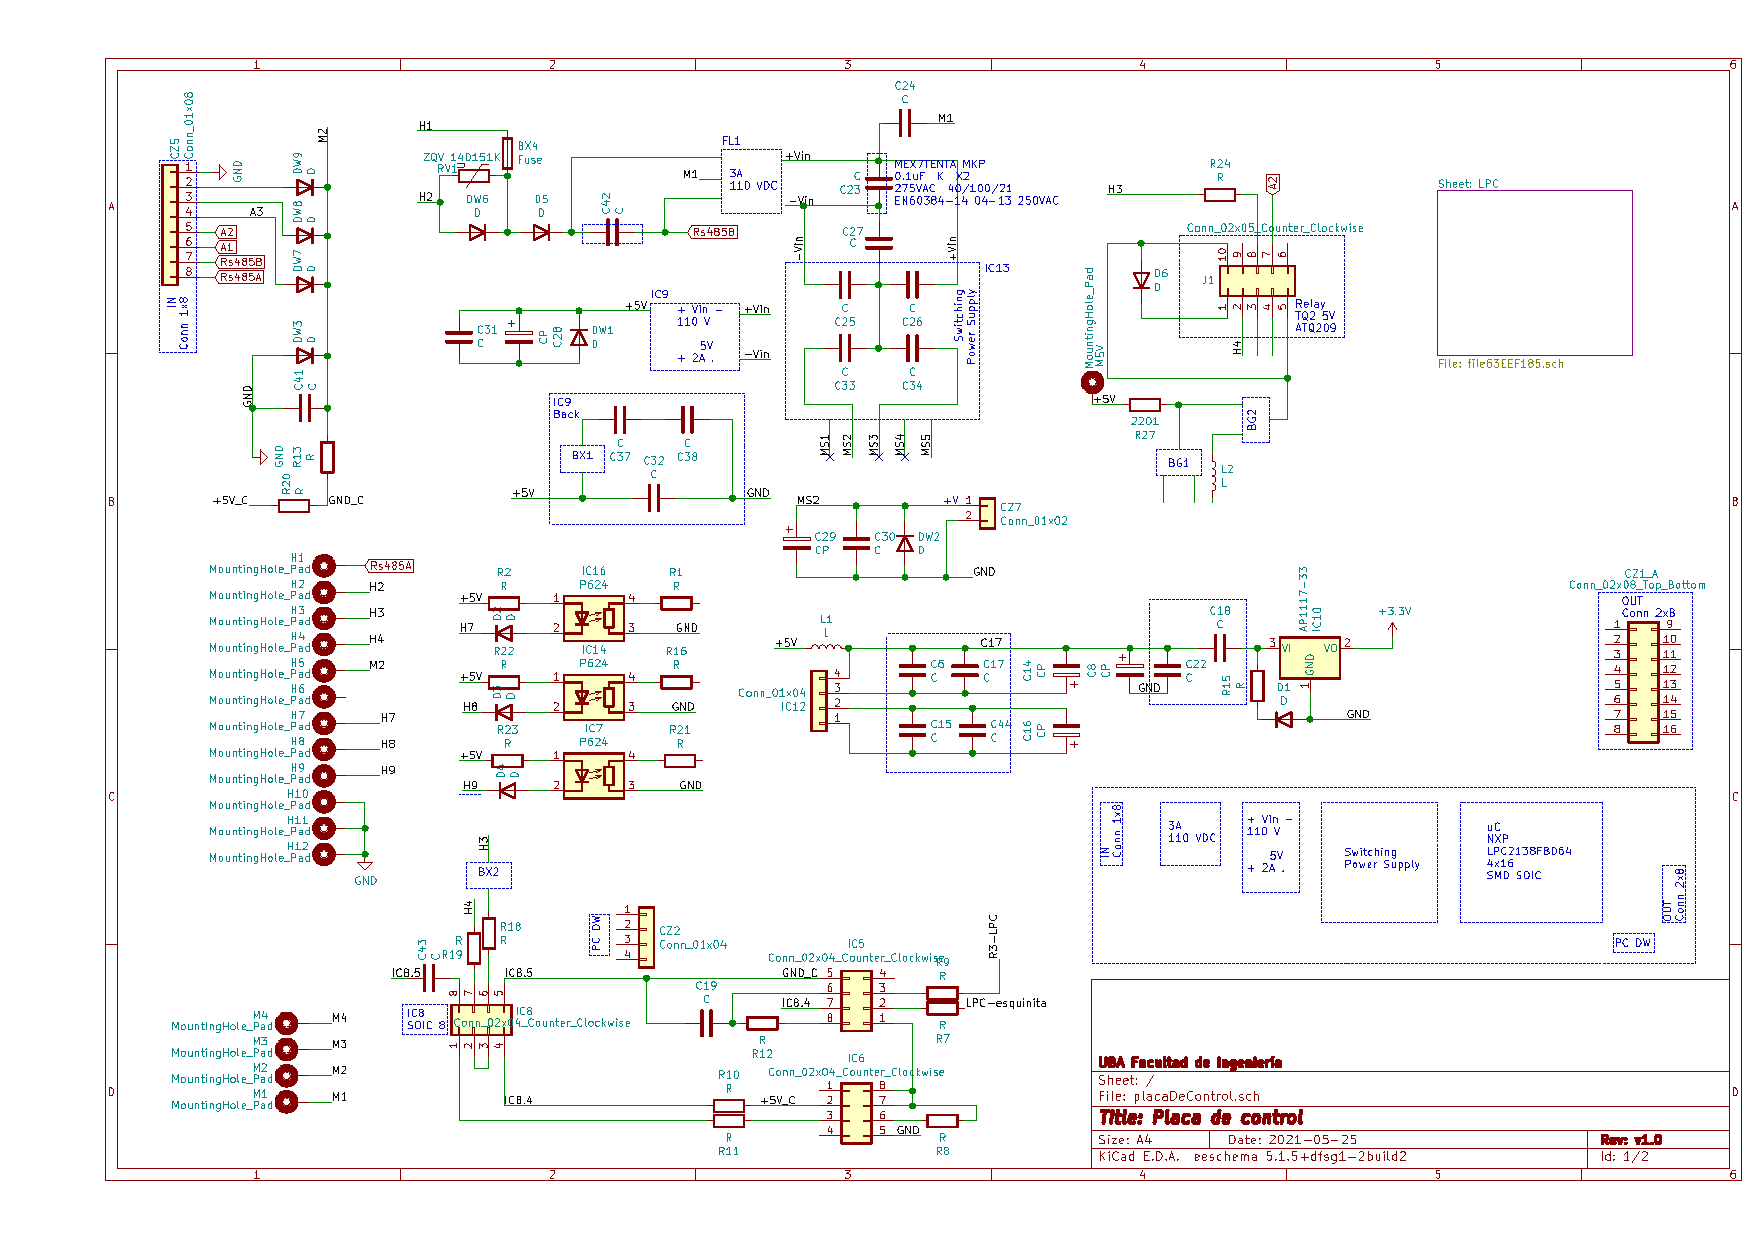
\includegraphics[width=1.66\textwidth, angle=90]{./Figures/output.placaControl.pdf}
	\caption{Circuito esquemático de la placa de control de los carteles LED de salón.}
	\label{fig:schController}
\end{figure}
%\include{Appendices/AppendixB}
%\include{Appendices/AppendixC}

%----------------------------------------------------------------------------------------
%	BIBLIOGRAPHY
%----------------------------------------------------------------------------------------

\Urlmuskip=0mu plus 1mu\relax
\raggedright
\printbibliography[heading=bibintoc]

%----------------------------------------------------------------------------------------

\end{document}  
